% **************************************************
% Document Class Definition
% **************************************************
\documentclass[%
    paper=A4,               % paper size --> A4 is default in Germany
    ngerman,
    twoside=true,           % onesite or twoside printing
    openright,              % doublepage cleaning ends up right side
    parskip=half,           % spacing value / method for paragraphs
    chapterprefix=true,     % prefix for chapter marks
    11pt,                   % font size
    headings=normal,        % size of headings
    bibliography=totoc,     % include bib in toc
    listof=totoc,           % include listof entries in toc
    titlepage=on,           % own page for each title page
    captions=tableabove,    % display table captions above the float env
    chapterprefix=false,    % do not display a prefix for chapters
    appendixprefix=false,    % but display a prefix for appendix chapter
    draft=false,            % value for draft version
]{scrreprt}%

% **************************************************
% Setup YOUR thesis document in this file !
% **************************************************

\usepackage[table]{xcolor}
\usepackage{algorithm}
%\usepackage{algorithmic}
\usepackage{algpseudocode}
\input{my-thesis-setup}


% **************************************************
% Document CONTENT
% **************************************************
\begin{document}

\renewcommand{\an}[1]{\textbf{\textcolor{red}{AN: #1}}}
% uncomment the following command to fill up pages with
% whitespace instead of aligning the first and last lines
% of a page (see \raggedbottom vs. \flushbottom)
%\raggedbottom

% --------------------------
% rename document parts
% --------------------------
\renewcaptionname{ngerman}{\figurename}{Abb.}
\renewcaptionname{ngerman}{\tablename}{Tab.}
%\renewcaptionname{english}{\figurename}{Fig.}
%\renewcaptionname{english}{\tablename}{Tab.}

% --------------------------
% Front matter
% --------------------------
\pagenumbering{roman}			% roman page numbering (invisible for empty page style)
\pagestyle{empty}				% no header or footers
% !TEX root = ../my-thesis.tex
%
% ------------------------------------  
% ------------------------------------  
% --> cover title page
% THIS PAGE IS NOT REQUIRED BUT MIGHT BE USEFUL IF 
% ------------------------------------  
% ------------------------------------  
\ifShowExtraTitlePage % use this flag for enabling or disabling this extra cover page
\begin{titlepage}
        \todo[inline]{Diese Seite kann mit ShowExtraTitlePagefalse deaktiviert werden.}
	\pdfbookmark[0]{Cover}{Cover}
	\flushright
	\hfill
	\vfill
	{\LARGE\thesisTitle \par}
	\rule[5pt]{\textwidth}{.4pt} \par
	{\Large\thesisName}
	\vfill
	\textit{\large\thesisDate} 
    \ifShowVersionOnExtraTitlePage        
        \\
	Version: \thesisVersion
        \todo[inline]{Versionsdarstellung kann mit ShowVersionOnExtraTitlePagefalse deaktiviert werden.}
    \fi
\end{titlepage}
\fi

% ------------------------------------  --> main title page
\begin{titlepage}
	\pdfbookmark[0]{Titlepage}{Titlepage}
	\tgherosfont
	\centering

	%{\Large \thesisUniversity} \\[4mm]
        %  trim={left bottom right top},clip
	
\includegraphics[width=6cm,trim={0 3cm 0 0},clip]{gfx/logos/HTWK_Zusatz_de_V_Black_K.eps} \\[2mm]
	\textsf{\thesisUniversityDepartment} \\
	%\textsf{\thesisUniversityInstitute} \\
	%\textsf{\thesisUniversityGroup} \\

	\vfill
	{\large \thesisSubject} \\[4mm]
	{\LARGE \color{ctcolortitle}\textbf{\thesisTitle} \\[10mm]}

    % \an{This title is too long and does not fit. Better: Multilingual Question Answering on Knowledge Graphs}
	{\Large \thesisName} \\[15mm]
%\textsf{to the} \\
%{Faculty of Computer Science, Electrical Engineering and Mathematics} \\
%\textsf{of}\\
%{Paderborn University}\\
%\textsf{}\\ INFO: removed because not necessary
%\textsf{Abschlussarbeit zur Erlangung des akademischen Grades\\Master of Science (M.\,Sc.)}\\
{}
	\vfill
	\begin{minipage}[t]{.27\textwidth}
		\raggedleft
		\textit{Betreuer}
	\end{minipage}
	\hspace*{15pt}
	\begin{minipage}[t]{.65\textwidth}
		{\large \thesisFirstReviewer} \\
	  	{\small \thesisFirstReviewerDepartment} \\[-1mm]
		{\small \thesisFirstReviewerUniversity}
	\end{minipage} \\[4mm]
    % INFO: removed because there is only 1 reviewer
	% \begin{minipage}[t]{.27\textwidth}
	% 	\raggedleft
	% 	\textit{2. Betreuer}
	% \end{minipage}
	% \hspace*{15pt}
	% \begin{minipage}[t]{.65\textwidth}
	% 	{\large \thesisSecondReviewer} \\
	%   	{\small \thesisSecondReviewerDepartment} \\[-1mm]
	% 	{\small \thesisSecondReviewerUniversity}
	% \end{minipage} \\[4mm]
 %        \begin{minipage}[t]{.27\textwidth}
	% 	\raggedleft
	% 	\textit{3. Betreuer}
	% \end{minipage}
	% \hspace*{15pt}
	% \begin{minipage}[t]{.65\textwidth}
	% 	{\large \thesisThirdReviewer} \\
	%   	{\small \thesisThirdReviewerDepartment} \\[-1mm]
	% 	{\small \thesisThirdReviewerUniversity}
	% \end{minipage} \\ [4mm]
%	\begin{minipage}[t]{.27\textwidth}
%		\raggedleft
%		\textit{Supervisors}
%	\end{minipage}
%	\hspace*{15pt}
%	\begin{minipage}[t]{.65\textwidth}
%		\thesisFirstSupervisor \\  \thesisSecondSupervisor
%	\end{minipage} \\[5mm]
        \vspace*{4ex}
	\begin{minipage}[t]{.27\textwidth}
		\raggedleft
		\textit{Einreichungsdatum:}
	\end{minipage}
	\hspace*{15pt}
	\begin{minipage}[t]{.65\textwidth}
	  	{\small \thesisDate}
	\end{minipage} \\[4mm]
    \todoinline{Diese Seite kann in der Datei \texttt{my-thesis-setup.tex}\ konfiguriert werden.}
\end{titlepage}


% ------------------------------------  --> lower title back for single page layout
\hfill
\vfill
{
    \small
    \textbf{\thesisName} \\
    \textit{\thesisTitle} \\
    \thesisSubject, \thesisDate \\
    Betreuer: \thesisFirstReviewer\\[1.5em]
    \textbf{\thesisUniversity} \\
    \textit{\thesisUniversityGroup} \\
    \thesisUniversityInstitute \\
    \thesisUniversityDepartment \\
    \thesisUniversityStreetAddress \\
    \thesisUniversityPostalCode\ \thesisUniversityCity
    \todoinline{Diese Seite kann in der Datei \texttt{my-thesis-setup.tex}\ konfiguriert werden. Hinweisboxen werden durch \Verb"\presetkeys{todonotes}{disable}{}" in der Präamble deaktiviert.
    Weitere Hilfen sind unter \href{https://wse-research.org/static-content/documents/Handout\%20-\%20Hinweise\%20zu\%20Ausarbeitung\%20einer\%20Abschlussarbeit\%20-\%20Andreas\%20Both.pdf}{https://wse-research.org/static-content/documents/Handout\%20-\%20Hinweise\%20zu\%20Ausarbeitung\%20einer\%20Abschlussarbeit\%20-\%20Andreas\%20Both.pdf} abrufbar.}
}
		% INCLUDE: all titlepages
% \cleardoublepage

\pagestyle{plain}				% display just page numbers
%
% !TEX root = ../my-thesis.tex
%
\pdfbookmark[0]{Kurzfassung}{Kurzfassung}
\addchap*{Kurzfassung}
\label{sec:kurzfassung}
\selectlanguage{ngerman}
\blindtext[2] % remove

\controlquestions{
\begin{enumerate}
    \item Wurde ein kompletter Überblick über die Arbeit und die jeweils wichtigsten Anforderungen, Ziele, Vorgehen, Ergebnisse und Erkenntnisse geben?
    \item Wurde ca. eine A4-Seite genutzt?
\end{enumerate}
} % INCLUDE: kurzfassung
% \cleardoublepage#
% !TEX root = ../my-thesis.tex
%
\pdfbookmark[0]{Abstract}{Abstract}
\addchap*{Abstract}
\label{sec:abstract}
\selectlanguage{english}
\kant[1-2] % remove

\controlquestions{
\begin{enumerate}
    \item Sind die deutschen Fachbegriffe passend und präzise in die englische Sprache übersetzt?
\end{enumerate}
}		% INCLUDE: the abstracts (english and german)
% \cleardoublepage
% % !TEX root = ../my-thesis.tex
%
\pdfbookmark[0]{Danksagung}{Danksagung}
\addchap*{Danksagung}
\label{sec:acknowledgement}

\blindtext[1] % remove

\controlquestions{
Dieser Abschnitt bietet die Möglichkeit, Personen oder Institutionen für ihre Unterstützung zu danken, sei es fachlich, finanziell, organisatorisch oder persönlich. 
Auch wenn dieser Abschnitt nicht bewertet wird, sollte er angemessen, respektvoll und professionell formuliert sein.
\begin{enumerate}
    \item Ist der Ton respektvoll, professionell und dankbar – ohne Übertreibung oder Ironie?
    \item Sind keine kritischen, wertenden oder unangemessenen Formulierungen enthalten?
    \item Sind alle genannten Namen und Titel korrekt geschrieben und verwendet (inkl. akademischer Titel, falls erforderlich)?
\end{enumerate}
}
 % INCLUDE: acknowledgement
% \cleardoublepage
\addchap*{Selbstständigkeitserklärung}

%\color{hsadarkgrayblue}{
%	\Headerfamily\bfseries\LARGE{}Selbstständigkeitserklärung
%}

\color{black}
\vspace{10mm}

Hiermit erkläre ich, dass die Arbeit selbstständig verfasst, in gleicher oder ähnlicher Fassung noch nicht in einem anderen Studiengang als Prüfungsleistung vorgelegt wurde und keine anderen, als die angegebenen Hilfsmittel und Quellen, einschließlich der angegebenen und beschriebenen Software, verwendet wurden.
%
\vspace{20mm}

\begin{minipage}{\linewidth}
%\fbox{
	\begin{minipage}{.30\linewidth}
		\underline{
			\makebox[.9\linewidth]{
				\mbox{
					Leipzig, \thesisDate
				}\hfill
			}
		}
		\makebox[.9\linewidth]{
			\mbox{\centering\small{Ort, Datum}}
		}
	\end{minipage}
%}
	\hfill
%\fbox{
	\begin{minipage}{.65\linewidth}
		\underline{
			\makebox[.9\linewidth]{
				\phantom{Leipzig, \thesisDate}\hfill
			}
		}
		\makebox[.9\linewidth]{
			\mbox{\small{Unterschrift der einreichenden Person}}\hfill
		}
	\end{minipage}	
%}
\end{minipage}

\vspace{20mm}

\ifShowSperrvermerk
{%\color{bblue}{
	\bfseries\LARGE{}Sperrvermerk
%}
}

\color{black}
\vspace{10mm}

\begin{minipage}{\linewidth}
%\fbox{
	\begin{minipage}{.35\linewidth}
        \ 
	\end{minipage}
%}
%\fbox{
	\begin{minipage}{.3\linewidth}
		Ja
		\ifthenelse{
			\equal{True}{\istgesperrt}
		}{
			\fbox{\mbox{\Huge{X}}}
		}{
			\fbox{\mbox{\phantom{\Huge{X}}}}
		}
	\end{minipage}
%}
%\fbox{
	\begin{minipage}{.3\linewidth}
		Nein
		\ifthenelse{
			\equal{True}{\istgesperrt}
		}{
			\fbox{\mbox{\phantom{\Huge{X}}}}
		}{
			\fbox{\mbox{\Huge{X}}}
		}
	\end{minipage}
%}
\end{minipage}

\vspace{5mm}

\ifthenelse{
	\equal{\CompanyName}{}
}{
	\def\sperrtext{Der Inhalt dieser Arbeit darf Dritten ohne Genehmigung von \erstergutachter~ nicht zugänglich gemacht werden. Dieser Sperrvermerk gilt für die Dauer von \sperrdauer~Jahren.}
}{
	\def\sperrtext{Der Inhalt der Arbeit darf Dritten ohne Genehmigung der/des \namedesunternehmens~nicht zugänglich gemacht werden. Dieser Sperrvermerk gilt für die Dauer von \sperrdauer~Jahren.}
}

\ifthenelse{
	\equal{True}{\istgesperrt}
}{
	\sperrtext
}{
}


\vspace{20mm}

\begin{minipage}{\linewidth}
%\fbox{
	\begin{minipage}{.30\linewidth}
		\underline{
			\makebox[.9\linewidth]{
				\mbox{
					Leipzig, \thesisDate
				}\hfill
			}
		}
		\makebox[.9\linewidth]{
			\mbox{\centering\small{Ort, Datum}}
		}
	\end{minipage}
%}
	\hfill
%\fbox{
	\begin{minipage}{.65\linewidth}
		\underline{
			\makebox[.9\linewidth]{
				\phantom{Leipzig, \thesisDate}\hfill
			}
		}
		\makebox[.9\linewidth]{
			\mbox{\small{Unterschrift der betreuenden Person des  Unternehmens \CompanyName}}\hfill
		}
	\end{minipage}	
%}
\end{minipage}
\fi

% \controlquestions{
% \begin{enumerate}
%     \item Wurde die Arbeit bei einem Unternehmen durchgeführt? (\texttt{ifShowSperrvermerk} konfigurieren)
% \end{enumerate}
% }

\vspace{60mm} % INCLUDE: Selbstständigkeitserklärung
% \cleardoublepage
%
\currentpdfbookmark{\contentsname}{toc}
\setcounter{tocdepth}{2}		% define depth of toc
\renewcommand{\contentsname}{Inhaltsverzeichnis} % remove if English thesis
\tableofcontents				% display table of contents
% \cleardoublepage

% --------------------------
% Body matter
% --------------------------
\pagenumbering{arabic}			% arabic page numbering
\setcounter{page}{1}			% set page counter
\pagestyle{scrheadings}			% header and footer style

% --------------------------
% Content
% --------------------------
% INFO: Todo Liste
\input{content/01_todos}
% INFO: Temporary Note chapter
% \chapter{Notizen, Struktur}\label{ch:Notizen}

\begin{tcolorbox}[colback=yellow!10!white, colframe=red!75!black, title=\textbf{PROJEKT NOTIZEN}]
Hier werden zunächst nur grobe Notizen / Informationen gesammelt. Diese binden bereits BibTex Zitationen mit ein, sind aber nur grob sortiert.

\textbf{Hinweis:} Die Struktur dieses Kapitels spiegelt \textbf{nicht} die echte Struktur dieser Arbeit wieder. Es handelt sich hier nur um eine Sammlung von Themenkomplexen.
\end{tcolorbox}

Forschungsfragen des Masterprojektes:\todo[inline]{Forschungsfragen kommen in Ch.1, Erläuterung sollte folgen.}

\begin{description}
    \item[RQ1]\label{RQ1} Wie kann aus Userstories passender funktionaler Quellcode und zugehöriger Text erzeugt werden?
    \item[RQ2]\label{RQ2} Wie hoch ist der Automatisierungsgrad?
\end{description}

Zunächst die grobe Unterteilung in die einzelnen Themenbereiche, die für diese Arbeit betrachtet werden sollen. Hier werde ich zunächst Notizen zu bestimmten Papers/Arbeiten sammeln, damit ich die Citations bereits einfügen kann.

% ##################################### SUBSECTION #####################################

\subsection{Generelle Informationen}

Die Forschungsfragen \ref{RQ1} und \ref{RQ2} sollen in dieser Arbeit hinsichtlich des aktuellen Forschungsstandes beantwortet werden. Zur Sammlung von relevanten wissenschaftlichen Arbeiten lehne ich mich an \cite{kitchenhamGuidelinesPerformingSystematic2007} an, welches primär für Systematische Literatur Reviews geschrieben wurde.

Die Idee ist hier einen Prozess zu definieren, anhand relevante Arbeiten gesammelt und konzentriert werden. Die dabei wichtigesten \textasciitilde 20 Arbeiten werden gesammelt und analysiert. Damit soll in Kapitel \ref{ch:Verwandte Arbeiten} eine konkrete Analyse und Aufarbeitung dieser Arbeiten geschehen. Hier werden auch Arbeiten zu gleichen Themenbereichen gegenüber gestellt und verglichen.

Unabhängig von diesem Prozess habe ich selbständig relevante wissenschaftliche Arbeiten gesucht, welche in den Prozess mit eingebunden werden.

\subsubsection{Informationsbeschaffung wissenschaftlicher Literatur}

Wie bereits angeführt soll im Ramen dieser Arbeit eine Analyse vorhandener Literatur stattfinden. Dabei ergeben sich Thematische Schwerpunkte welche der direkten Beanwortung der Forschungsfragen dienen:

\begin{itemize}
    \item Generierung von Quellcode aus Anforderungen
    \item Automatisierungsgrad von LLM (Multi-Agent) Systemen \textit{(für Quellcode Generierung)}
\end{itemize}

Weiterhin gibt es verschiedene Themenkomplexe welche durch ihre unmittelbare Nähe zu den Forschungsfragen \textit{oberflächlich} analysiert werden sollen:

\begin{itemize}
    \item Quellcode Generation durch Multi-Agent Systeme
    \item Generation von User Stories
    \item Generation von Tests (Unit, E2E, Integration, UAT)
    \item Evaluation von Ergebnissen (LLM-Judges, etc.)
\end{itemize}

\subsubsection{Meta Analyse}

Hier soll zunächst die Outline für eine Meta Analyse definiert werden. Fokus der Analyse ist es, möglichst relevante wissenschaftliche Arbeiten zu sammeln und zu analysieren. Hinsichtlich des vorherigen Unter-Kapitels und in Betrachtung der Empfehlungen von \cite{kitchenhamGuidelinesPerformingSystematic2007} verfolge ich folgende Strategie:

\begin{enumerate}
    \item Definition von Inklusions/Exklusions-Kriterien
    \item Schlüsselwort Sammlung, daraus Queries definieren
    \item Sammlung durch akademische Tools (IEEExplore, arXiv, etc.)
    \item Bündelung und Sortierung von Ergebnissen
    \item Filtern der Ergebnisse
\end{enumerate}

Nach diesem Prozess sollten sich ca \textasciitilde 20 wissenschaftliche Arbeiten mit starker Relevanz ergeben.

\subsubsection{Umsetzung Meta Analyse}

\textbf{Strategie 1: SLR ähnliche Analyse via IEEExplore}

\begin{enumerate}
    \item Definition einer Query
    \item Anwendung Inclusion Criteria (IC)
    \item Anwendung Exclusion Criteria (EC)
    \item Screening (Manual?=)
\end{enumerate}

\textbf{Query}

Um möglichst viele Paper auf einmal zu gewinnen wird eine Query via IEEE Xplore ausgeführt. Hier wird bereits ein IC angewendet, da IEEE Xplore diese Funktionalität Diese sieht wie folgt aus:

\begin{verbatim}
    ("Large Language Model" OR LLM OR "Generative AI") 
    AND ("User Story" OR Requirement) 
    AND ("Code Generation" OR Autonomous OR "Multi-Agent")
\end{verbatim}
= 524 Arbeiten

\textbf{Inclusion Criteria / Inklusionskriterien}

\begin{enumerate}
    \item Publikation zwischen 2023 und 2026
    \item Arbeit behandelt die Transformation von natürlichsprachlich formulierten Anforderungen in Quellcode
    \item Arbeit nutzt LLMs / Agentic Frameworks / Multi-Agent-Systeme
    \item Arbeit evaluiert ihre Ergebnisse oder beschreibt die Architektur des Systems (am besten auch den Grad der Automatisierung)
\end{enumerate}

\begin{figure}
    \centering
    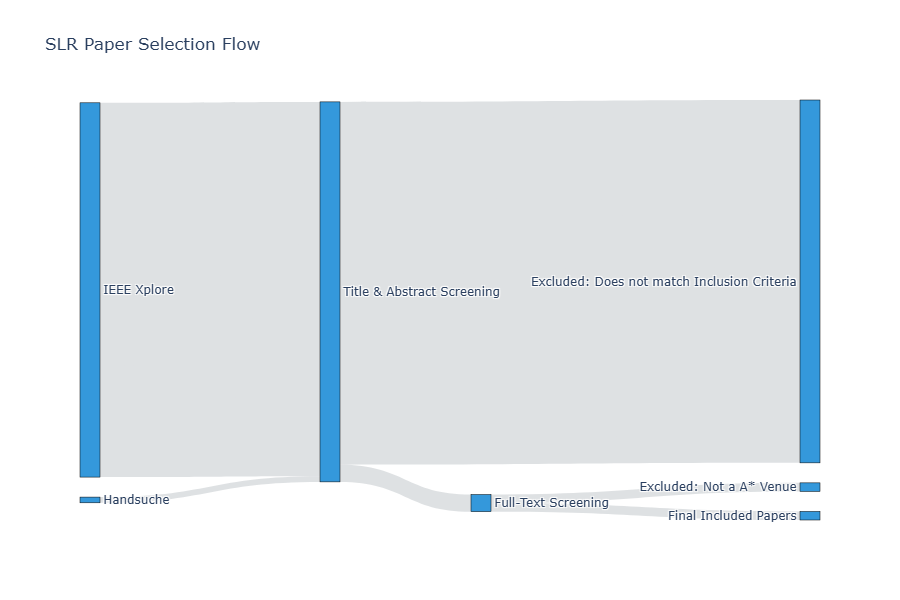
\includegraphics[width=1\linewidth]{images/selection_plot.png}
    \caption{Auswahl der Arbeiten}
    \label{fig:paper_selection}
\end{figure}

% \begin{enumerate}
%     \item Thematische Abarbeitung der Abstracts nach den IC:
%     \begin{enumerate}
%         \item Publikation zwischen 2023 und 2026
%         \item Arbeit behandelt die Transformation von natürlichsprachlich formulierten Anforderungen in Quellcode
%         \item Arbeit nutzt LLMs / Agentic Frameworks / Multi-Agent-Systeme
%         \item Arbeit evaluiert ihre Ergebnisse oder beschreibt die Architektur des Systems (am besten auch den Grad der Automatisierung)
%     \end{enumerate}
% \end{enumerate}

\textbf{Vorgehen}

\subsection{User Stories \& Requirements Engineering}

\subsubsection{User Acceptance Testing}

\cite{varpeUserAcceptanceTest2025} extrahiert aus Anforderungsdokumenten direkt User Acceptance Tests (UAT).\todo[inline]{Klären wie Acronyms zu behandeln sind! Glossary am Ende der Arbeit?} 
Die Idee selbst ist nicht neu, es wurde beispielsweise bereits aus UML-Diagrammen und XML Daten UAT generiert, dies erfordert allerdings einen weiteren Prozessschritt zur Aufbereitung der Anforderungen. Dieser Prozess lässt sich wie in \cite{varpeUserAcceptanceTest2025} gezeigt wird, auch mit einer LLM basierten Methodologie umsetzen, wobei echte Anforderungsdokumente aus \cite{ferrariPUREDatasetPublic2017a} als Testdaten dienen. Ein System aus 2 LLM-Agenten genügt hier für vielversprechende Ergebnisse.

\textbf{Aber:} Die Methodologie des Papers ist nicht unbedingt 100\% klar. Die Bewertung der Ergebnisse erfolgt via LLM-As-A-Judge und behauptet eine Coverage der Anforderungen von bis zu 72\%. Eine (heuristische?) Analyse via BERTScore wurde nur auf \textbf{1} Beispiel ausgeführt.

\textbf{Extra Note:} der Datensatz aus \cite{ferrariPUREDatasetPublic2017a} ist nicht uninteressant, da es hier eine große Menge and Anforderungen gibt die man evtl. für andere Zwecke nutzen kann. 

\subsection{Software Design}

\subsection{Code Generation}

\subsection{Automatisierung von Quellcode Generation}

\subsection{Evaluation von Resultaten}

Um die Ergebnisse von verschiedenen LLMs und Lösungsansätzen für NL2Code vergleichen zu können, bedarf es Benchmarks. In Benchmarks werden... 

\subsubsection{Herausfoderungen akurater Bewertung}



\subsubsection{Kontamination von Datensätzen}

Eine weitere gravierende Herausforderung für Benchmarks ist die Kontimination der Datensätze. Moderne LLMs werden auf massiven Datenmengen trainiert. Wenn ein Benchmark auf Open Source Projekten basiert, ist es praktisch unvermeidbar dass diese Projekte ebenfalls in die Testdaten mit eingehen. 

\todo[inline]{Kontamination ist nicht das richtige Wort, außerdem braucht es heir eine Primärquelle für das Problem selbst. --> Overfitting?}

% --------------------------------------------------------------------------------------------
% --------------------------------------------------------------------------------------------
% --------------------------------------------------------------------------------------------

\todo[inline]{Ab hier test Sektion für Formattierung, etc.}

\cleardoublepage

% TODO: Commented out because not yet required + to reduce compile times
% !TEX root = ../my-thesis.tex
%
\chapter{Motivation und Problemdefinition}\label{ch:Motivation und Problemdefinition}

\todo[inline,color=red!80]{Ob hier ein Section Header hinmuss oder nicht gilt zu klären, evtl. ist es schöner ohne? Oder einfach in 2 Teilen, pures Intro ohne und dann Automatisierung und so (siehe TODO unten) unter section\{Ausgangslage\}}
% \section{Ausgangslage}\label{ch:Ausgangslage}

Die Softwareentwicklung ist mehr denn je durch Anforderungen getrieben. Um dieser Notwendigkeit gerecht zu werden, wurde das Themengebiet des ''Requirements Engineering'' (RE) ins Leben gerufen, das bis zum heutigen Stand von einer starken Mehrheit der Entwickler als ''sehr wichtig'' empfunden wird.\cite{wangRoleRequirementsEngineering2014} Um der stets steigenden Menge an Anforderungen gerecht zu werden, ist die meistverbreitetste Methode, um Anforderungen darzustellen und zu dokumentieren, die ''User Story''\cite{wangRoleRequirementsEngineering2014}. Oft im originellen Format nach [...]\todo{cite} ist sie wie folgt definiert:

''As a \textlangle \textit{role}\textrangle, I want a \textlangle \textit{goal}\textrangle, [so that \textlangle \textit{benefit}\textrangle].''

Unter der Annahme, dass diese strukturiert und bewusst eingesetzt werden, stellen sie für viele Entwickler ein nützliches und produktivitätssteigerndes Werkzeug dar.\cite{lucassenUseEffectivenessUser2016}

Im Zeitalter von Large Language Models (LLMs) und agentischen Entwicklungsverfahren ist es so leicht wie nie zuvor, Quellcode aus Natürlichssprachigen Anforderungen zu erzeugen. Neben den bist dato stets steigenden Kapazitäten von LLMs diese Aufgabe (auch NL2Code genannt) zu lösen werden auch stets neue Benchmarks entworfen um diese Fähigkeiten gegenüber möglichst realistischen Bedienungen zu prüfen.\cite{jiangSurveyLargeLanguage2026} Dabei wird auffällig, dass Anforderungen oft, entgegen den Erkentnissen aus dem RE, in massiven Text-Korpusen integriert werden.

\todo[inline]{Weiterer Einstieg zur Automatisierung von Prozessen notewendig}

\section{Problemdefinition}\label{ch:Problemdefinition}

Die Frage die sich nun stellt ist ob die Verwendung von User-Stories für die Generierung von Quellcode nützlich ist. Doch hierfür muss zuerst der aktuelle Stand der Wissenschaft in Hinsicht auf die NL2Code Aufgabe analysiert und verstanden werden.

Hierbei ergeben sich mehrere Probleme, die es in dieser Arbeit zu betrachten gilt:

\begin{itemize}
    \item Vorhandene Arbeiten berichten ihre Ergebnisse oft unter eigenen Bedienungen (Beispielsweise Modelle, Hyperparameter, RAG-Strategien, Metriken und Benchmarks).
    \item Daher ist es oft nicht möglich diese Ergebnisse untereinander zu vergleichen.
    \item Aussagen zum Automatisierungsgrad sind generell heterogen und nicht vergleichbar.
\end{itemize}

Diese Gesichtspunkte machen es äußerst schwer die Fragen aus unser ursprünglichen Problemdefinition zu beantworten.

\section{Zielsetzung und Forschungsfragen}\label{ch:Zielsetzung und Forschungsfragen}

Ziel dieser Arbeit ist es, unter angesicht der oben genannten Probleme bestehende wissenschaftliche Arbeiten zu untersuchen und diese in Hinsicht auf die NL2Code Aufgabe einzuordnen und zu vergleichen. Hierzu wird der Stand der Grundlagen sowie aktuelle Lösungsansätze genauer betrachtet. Die Fragen und die Thematik stammen dabei von der Forschungsgruppe WSE, aufzufinden unter \cite{WSEResearchThema}. Die Arbeit fokussiert sich exlpizit auf folgende 2 Forschungsfragen:

\begin{description}
    \item[RQ1]\label{RQ1} \textbf{Wie kann aus Userstories passender funktionaler Quellcode und zugehöriger Text erzeugt werden?}
\end{description}

Es gilt zu untersuchen inwiefern LLMs in der Lage sind, User Stories (in natürlicher Sprache) in funktionsfähigen Quellcode zuzuwandeln. Folglich muss analysiert werden wie gut LLMs mit aktuellen Lösungsansätzen in der Lage sind die Anforderungen von User Stories zu interpretieren und darauf basierend vollständigen, syntaktisch korrekten funktionsfähigen Quellcode zu generieren.

Weiterhin soll in diesem Umfang auch geprüft werden, wie gut diese Modelle erklärende Texte, wie Kommentare oder API-Dokumentationen, automatisch erstellen können.

\begin{description}
    \item[RQ2]\label{RQ2} \textbf{Wie hoch ist der Automatisierungsgrad?}
\end{description}

Diese Frage analysiert den Grad der Autoamtisierung, der bei der Generierung von Quellcode aus Userstories erreicht werden kann. Es wird untersucht, inwieweit der Prozess vollständig automatisiert durchgeführt werden kann, ohne dass manuelle Eingriffe erforderlich sind. 

Dabei wird auch betrachtet, in welchen Phasen der Code-Generierung oder -Anpassung menschliche Eingriffe besonders wichtig sind und wo die Grenzen der LLM-basierten Automatisierung liegen.

\section{Erfolgskriterien und Abgrenzung}\label{ch:Erfolgskriterien und Abgrenzung}

Das Ziel dieser Arbeit ist es wie bereits beschrieben die Grundlagen zu erläutern und den aktuellen Stand zu vermitteln. In Hinsicht auf \rqref{RQ1} ergeben sich dadurch folgende Ziele für diese Arbeit:

\begin{enumerate}
    \item $N$ Lösungsansätze werden gegen $M$ Benchmarks evaluiert
    \item Die Bedienung für diese Evaluationen sind dokumentiert und für alle Durchläufe möglichst identisch
    \item Abweichungen zu publizierten Werten werden quantifiziert
\end{enumerate}

Hierzu muss erwähnt werden, dass es zum heutigen Stand keinen Benchmark gibt der tatsächlich mit User-Stories arbeitet. Daher kann die Frage \rqref{RQ1} nicht in Hinsicht auf Userstories analysiert werden, da dies außerhalb des Rahmens dieser Arbeit liegt. Für die Frage \rqref{RQ2} ergibt sich weiterhin folgendes Ziel:

\begin{enumerate}
    \item Es existiert ein Klassifikationsschema für existierende Arbeiten, welches deren Automatisierungsgrad erkennbar macht
\end{enumerate}

Die Beantwortung von \rqref{RQ2} erfolgt im Gegensatz zu \rqref{RQ1} nicht via einem Experiment. Die Einordnung erfolgt vie Klassifikation anhand der Arbeiten, da diese bereits ein umfangreiches Bild darstellen.

\section{Forschungsprozess / Vorgehen}\label{ch:Forschungsprozess / Vorgehen}

Das weitere Vorgehen in dieser Arbeit sieht folgender maßen aus: Zuerst sollen relevante Arbeiten aus dem Themenfeld betrachtet werden. Zu diesem Zweck erfolgt eine Literaturaufarbeitung, angelehnt and SLR-Verfahren (aber skaliert auf den Umfang dieser Arbeit). Daraus folgt die Ableitung von eigenen Experimenten, die den aktuellen Stand der Forschung darstellen und vergleichen sollen. Aufbauend auf dieser Ableitung folgt die Konzeption und folgliche Implementierung eines Orchestrators. Dieser soll die letzendliche Durchführung der Experimente ermöglichem. Schlussendlich folgt eine Darstellung der Ergebnisse und eine Einordnung.

\section{Aufbau der Arbeit}\label{ch:Aufbau der Arbeit}

\todo[inline]{Hier kommt die Überblick über die Struktur der Arbeit. TODO für das Ende!}

% \todo[inline]{1. Initiale Einleitung}

% \todo[inline]{2. Themen Überführung zu SWE}

% \todo[inline]{3. Von SWE zur modernen Verwendung von User Stories}

% \todo[inline]{4. Ableitung bisheriger Erkentnisse auf Code Generation via Agentic Systems}

% \subsection{Forschungsfragen}\label{research_questions}

% Im Rahmen dieser Arbeit soll der mögliche Einfluß von User Stories auf die Generation von Quellcode untersucht werden. Hierzu wird der Stand der Grundlagen sowie aktuelle Lösungsansätze genauer betrachtet. Dabei fokussiert sich die Arbeit exlpizit auf folgende 2 Forschungsfragen:

% \todo[inline]{Der Text zu den Forschungsfragen kommt von der \href{https://wse-research.org/thesis_topic/user-stories-to-code}{WSE Website} und ist legedlich leicht umformuliert. Ob das so okay ist gilt zu klären.}

% \begin{description}
%     \item[RQ1]\label{RQ1} \textbf{Wie kann aus Userstories passender funktionaler Quellcode und zugehöriger Text erzeugt werden?}
% \end{description}

% Es gilt zu untersuchen inwiefern LLMs in der Lage sind, User Stories (in natürlicher Sprache) in funktionsfähigen Quellcode zuzuwandeln. Folglich muss analysiert werden wie gut LLMs mit aktuellen Lösungsansätzen in der Lage sind die Anforderungen von User Stories zu interpretieren und darauf basierend vollständigen, syntaktisch korrekten funktionsfähigen Quellcode zu generieren.

% Weiterhin soll in diesem Umfang auch geprüft werden, wie gut diese Modelle erklärende Texte, wie Kommentare oder API-Dokumentationen, automatisch erstellen können.

% \begin{description}
%     \item[RQ2]\label{RQ2} \textbf{Wie hoch ist der Automatisierungsgrad?}
% \end{description}

% Diese Frage analysiert den Grad der Autoamtisierung, der bei der Generierung von Quellcode aus Userstories erreicht werden kann. Es wird untersucht, inwieweit der Prozess vollständig automatisiert durchgeführt werden kann, ohne dass manuelle Eingriffe erforderlich sind. 

% Dabei wird auch betrachtet, in welchen Phasen der Code-Generierung oder -Anpassung menschliche Eingriffe besonders wichtig sind und wo die Grenzen der LLM-basierten Automatisierung liegen.

% \todo[inline]{Hier kommt die Überblick über die Struktur der Arbeit. TODO für das Ende!}

% % \cleanchapterquote{The grand aim of all science [is] to cover the greatest number of empirical facts by logical deduction from the smallest possible number of hypotheses or axioms.}{Albert Einstein \cite{barnett2005universe}}{}


% % \begin{figure}[p]
% %     \centering
% %     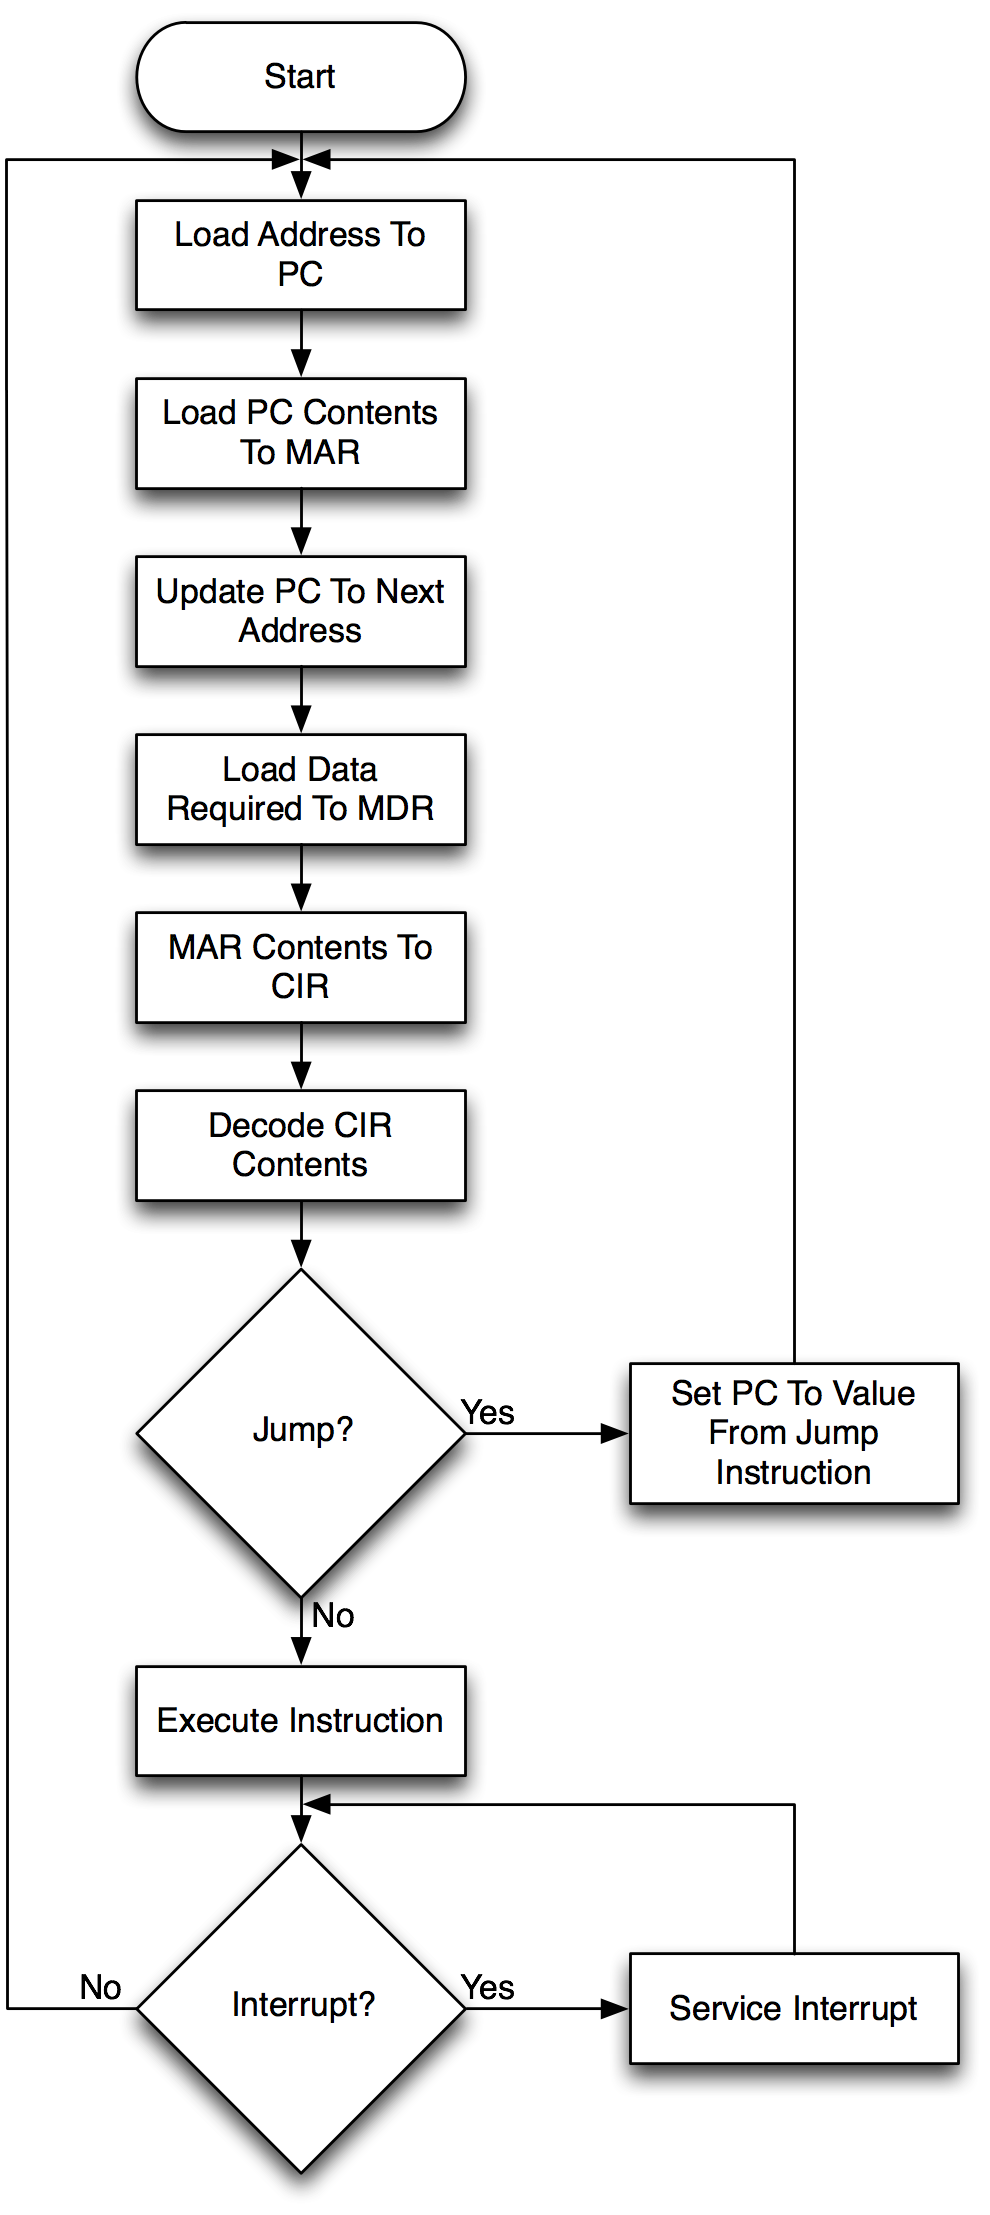
\includegraphics[height=\textheight]{images/Comp_fetch_execute_cycle.png}
% %     \caption{Every good research starts with a big picture describing the high-level research approach. \cite{WEB:flowchart_diagram}}
% %     \label{fig:big_picture}
% % \end{figure}

% % \lipsum[2-5] % remove 

% % \begin{figure}[t]
% %     \centering
% %     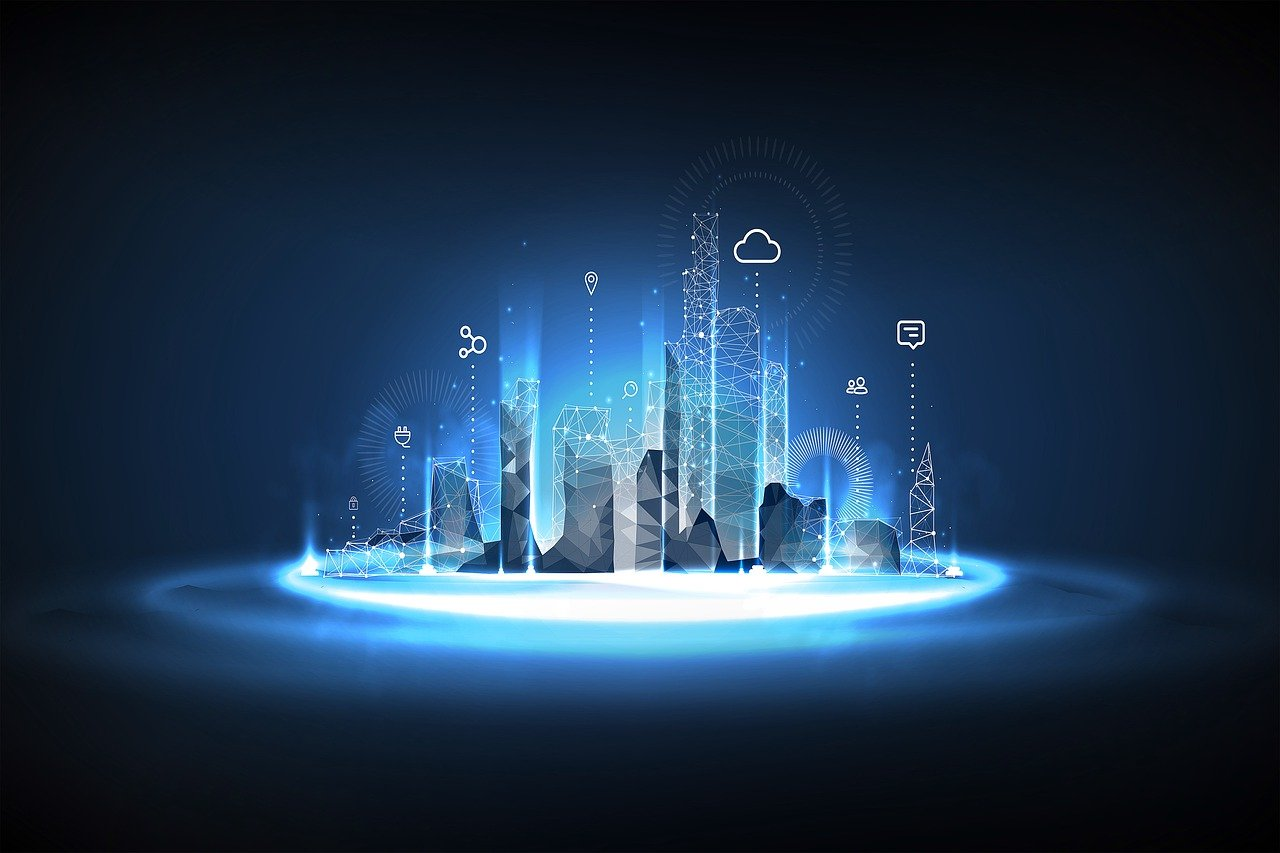
\includegraphics[width=.80\textwidth]{images/pixabay_technology-6701504_1280.jpg}
% %     \caption{Top-aligned image. \cite{PIXABAY:bild1}}
% %     \label{fig:image2}
% % \end{figure}

% % \lipsum[6-7] % remove 

% % \begin{description}
% %     \item[RQ1]\label{RQ1} ...
% %     \item[RQ2]\label{RQ2} ...
% %     \item[RQ3]\label{RQ3} ...
% %     \item[RQ4]\label{RQ4} ...
% % \end{description}

% % \lipsum[8-9] % remove 

% % \afterpage{ % Execute command after the next page break
% % \begin{landscape}
% % \begin{figure}
% %     \centering
% %     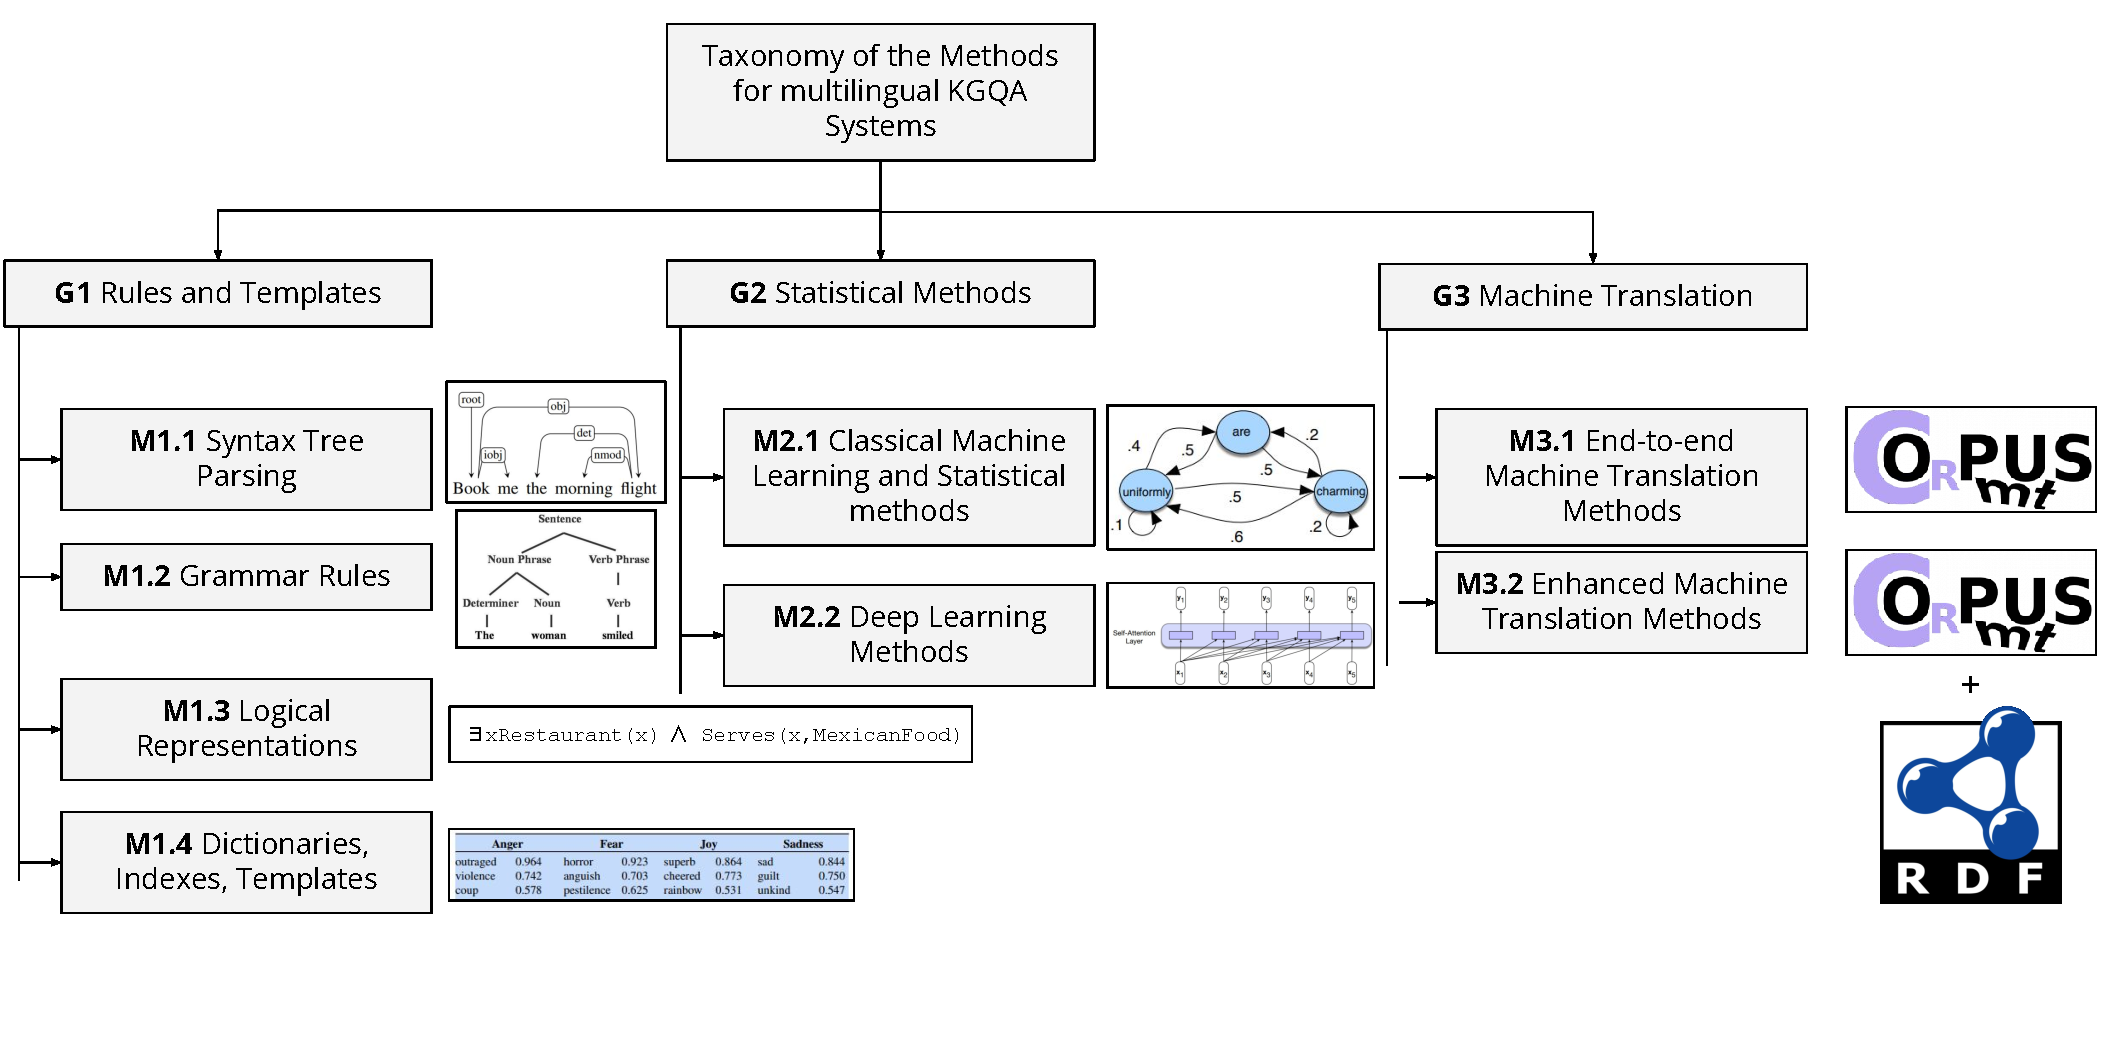
\includegraphics[width=\hsize]{gfx/taxonomy-multilingual-kgqa.pdf}
% %     \caption{An image in full landscape mode.}
% %     % source: https://docs.google.com/drawings/d/1M5NfSiLhNuRT3JuMr2WLTMpESCCnjup_Jok2EJlpzvI/edit?usp=sharing
% %     \label{fig:taxonomy}
% % \end{figure}
% % \end{landscape}
% % }

% % \lipsum[11-15] % remove 

% \controlquestions{
% \begin{enumerate}
%     \item Wurde eine Herleitung für das Thema vorgenommen (vom Allgemeinen, bis zum speziellen Themenbereich)?
%     \item Ist erkennbar, warum diese Arbeit besonders wichtig ist?
%     \item Wurde mindestens eine Forschungsfrage nachvollziehbar hergeleitet?
%     \item Wurde mindestens eine Forschungsfrage präzise formuliert?
%     \item Wurde der Ablauf (Forschungsprozess) der Arbeit dargestellt?
%     \item Wurde das messbare Erfolgskriterium benannt?
%     \item Wurde im letzten Abschnitt ein Überblick über die Struktur der Arbeit gegeben?
% \end{enumerate}
% }


\chapter{Theoretische Grundlagen und Begriffe}\label{ch:Theoretische Grundlagen und Begriffe}

Im Verlaufe dieser Arbeit werden etliche Begriffe aus dem Gebiet der Softwareentwicklung sowie Large Language Models benutzt. Dieses Kapitel dient der Erklärung der Grundlagen und der Begriffe aus diesen Gebieten.

\section{Software Engineering und Requirements Engineering}\label{ch:Software Engineering und Requirements Engineering}

Die Forschungsfrage \rqref{RQ1} erwähnt direkt zu Beginn den Begriff ''User Story''. Dieser Begriff stammt fundamental aus der Welt des Requirements Engineering; es bedarf damit also einer Einführung in diese Welt. 

\subsection{Requirements Engineering}\label{ch:Requirements Engineering}

Anforderungen (engl. Requirements) dienen als Grundlage von Software. Sie beschreiben in vielerlei Form die zugrundeliegenden Notwendigen Funktionen einer Software.\todo{Formulierung, evtl Citation} Bereits in den 70er Jahren wurde die Signifikanz von ''gut'' formulierten Anforderungen erkannt.\citeN{bellSoftwareRequirementsAre1976,boehmSoftwareEngineeringEconomics1984}. Um die Anforderungen an Software möglichst akkurat zu definieren, exisitiert das Themengebiet des \textbf{Requirement Engineering} (Kurz oft RE).

% Bereits 1976 erkannte \cite{bellSoftwareRequirementsAre1976} ein fundamentales Problem in der Softwareentwicklung: Die Ursachen eines Problems in Software zu lösen, ist leicht, wenn die Ursache im Code selbst liegt. Dies gilt ebenfalls für Defizite, die durch fehlerhaftes Design verursacht wurden. Diesen Fakten gegenüber steht das weitaus kompliziertere Problem: \textit{''If there are problems in developing requirements, however, the software system meeting those requirements will clearly not be effective in solving the basic need, even if the causes of the problems are incorrectly identified.''}\cite{bellSoftwareRequirementsAre1976}

% Die Signifikanz dieses Problems untermauern verschiedene Arbeiten aus der selben Zeit. Arbeiten wie \cite{boehmSoftwareEngineeringEconomics1984} schätzen die Kosten für eine späte Lösung von Requirements-basierten Problemen auf den Faktor 200 (Im Vergleich zu einer Lösung dieser Probleme in der Konzeptionsphase). Um gegen diese Probleme zu arbeiten und die Anforderungen an Software möglichst akkurat zu definieren, exisitiert das Themengebiet des \textbf{Requirement Engineering} (Kurz oft RE).

Die Prozesse des RE sind vielfältig, \cite{vanlamsweerdeRequirementsEngineeringYear2000} definiert beispielsweise folgende Gesichtspunkte:

\begin{itemize}
    \item Analyse der zugrunde-liegenden Domäne
    \item Erhebung von alternativen Modellen und Lösungen
    \item Verhandlung bzw. Evaluierung aller Lösungswege
    \item \textbf{Spezfikiation der letzendlichen Anforderungen und Annahmen}
    \item Analyse der definierten Spezifikationen in Hinsicht auf deren Genauigkeit und Umsetzbarkait
    \item Dokumentation der bestehenden Annahmen
    \item Evolution der definierten Anforderungen basierend auf neueren Erkentnissen oder Zielen
\end{itemize}

Im Sinne dieser Arbeit ist vor allem ein Punkt interessant: Die Spezifikation von Anforderungen.

\subsubsection{Funktionale und nicht-funktionale Anforderungen}\label{ch:Funktionale und nicht-funktionale Anforderungen}

Für unseren Rahmen gibt es verschiedene Arten von Anforderungen die wir zunächst erläutern sollten. 

\todo[inline]{FR und NFR hier erklären}

\subsection{User Stories}\label{ch:User Stories}

\todo[inline]{Buch link finden und dann hier erklären: Cohn, M.: User stories applied: for agile software development. Addison Wesley,  Redwood City (2004)}

Unterthemen die erwähnt werden sollten: Format, Akzeptanzkriterien, INVEST, Detailgrad und Ambiguität

\section{Large Language Models}\label{ch:Large Language Models}

\todo[inline]{Keine Wiederholung der Grundlagen - hier geht es um die Begriffe welche im Kontext verwendet werden}

Wichtige Begriffe:

\begin{itemize}
    \item Modell Größen, Parameter
    \item Modell Typen
    \item 
\end{itemize}

\todo[inline]{Evlt. auch kurze Historie, könnte aber besser in 4.0 aufgehoben sein.}

\section{Code Generierung (NL2Code)}\label{ch:Code Generierung (NL2Code)}

Fundamentale Grundlage dieser Arbeit ist die Generierung von Quellcode. Die Code-Generierung gilt es zunächst als Begriff in den groberen Themenbereich von Quellcode-nahen Aufgaben einzuordnen. Der Begriff wird ferner auch historisch im Bezug auf die Softwareentwicklung eingeordnet. Hier gilt es ebenfalls, LLMs in diesen Kontext einzuführen, da diese in der Gegenwart die relevantesten Werkzeuge für die Quellcodegenerierung darstellen.\todo[inline]{Cite the survey paper from 2025 which took this into account}

\todo[inline]{evtl \ref{ch:Einordnung des Begriffs} und \ref{ch:Historische Entiwcklung} tauschen. Macht vlt mehr Sinn? idk.}

\subsection{Einordnung des Begriffs}\label{ch:Einordnung des Begriffs}

Quellcode-Generierung wie sie in dieser Arbeit betrachtet wird, fokussiert sich ausschließlich auf die Aufgabe, Natürlich-sprachigen Text (NL) in Quellcode zu transformieren. Daher wird ab diesem Kapitel die Abkürzung ''NL2Code'' (Natural language to code, Natürliche Sprache zu Code) verwendet. 

\begin{table}[htbp]
    \centering
    % Erhöht den Zeilenabstand leicht für bessere Lesbarkeit
    \renewcommand{\arraystretch}{1.3} 
    
    % Spaltendefinition: l = linksbündig, p{Breite} = Blocksatz mit festem Umbruch
    \begin{tabular}{@{}lllp{8cm}@{}}
        \toprule
        \textbf{Typ} & \textbf{I-O} & \textbf{Aufgabe} & \textbf{Definition} \\
        \midrule
        
        % --- Bereich 1: Understanding ---
        \multirow{6}{*}{Verständniss} 
        & \multirow{4}{*}{C-K} 
        & Code Klassifizierung & Klassifizierung von Code-Schnipseln basierend auf deren Funktionalität, Zweck oder deren Attribute um bei der Organisation und Analyse zu helfen. \\
        & & Bug Detektion & Detektieren und Diagnostizieren von Bugs oder Vulnerabilities im Code, zur sicherstellung von Funktionalität und der Sicherheit. \\
        & & Klon Detektion & Identifizierung von Duplikaten oder ähnlichen Code Schnipseln um die Wartbarkeit zu verbessern, aber auch um Redundanzen zu entfernen und auf Plagiate zu überprüfen. \\
        & & Exception Type Detection & Vorhersage von Exception Typen im Code um diese zu managen und bessern zu handlen. \\
        \cmidrule{2-4}
        & C-C & Code-to-Code Retrieval & Abruf relevanter Code Schnipsel basierend auf gegebenen Code Queries für die Weiterverwendung oder Analyse \\
        \cmidrule{2-4}
        & NL-C & Code Suche & Abruf relevanter Code Schnipsel basierend auf natürlicher Sprache (NL) für die Weiterverwendung oder Analyse \\
        \midrule
        
        % --- Bereich 2: Generation ---
        \multirow{7}{*}{Generation} 
        & \multirow{5}{*}{C-C} 
        & Code Verfollständigung & Vorhersage und Vorschlagung der nächsten Code Sektion aus einem gegebenem Kontext. Dieser beinhaltet kontextuelle Information vom Prefix (und Suffix). Dient der Verbesserung in der Entwicklungsgeschwindigkeit und Genauigkeit. \\
        & & Code Übersetzung & Übersetzung von Code von einer Programmiersprache in eine andere, wobei Funktionalität und Logik erhalten bleiben. \\
        & & Code Reparatur & Identifizieren und Lösen von Bugs im Code durch Generierung einer korrekten Version. Verbessert damit Funktionalität und Verlässlichkeit.  \\
        & & Mutations Generation & Generierung von modifizierten Versionen von Code zur Evaluation von Test Strategien \\
        & & Test Generation & Generation von Tests um Code hinsichtlich seiner Funktion, Performance und Robustikgeit zu prüfen. \\
        \cmidrule{2-4}
        & C-NL & Code Zusammenfassung & Gerenierung von Text Beschreibungen (NL) von Code um Verständniss und Dokumentation zu verbessern. \\
        \cmidrule{2-4}
        & NL-C & Code Generation & Generation von Code aus NL um Entwicklungsprozesse zu streamlinen und manuellen Aufwand zu reduzieren \\
        \bottomrule
    \end{tabular}
    
    % Das optionale Argument in den eckigen Klammern ist für das Tabellenverzeichnis
    \caption[Anwendungsbereiche von Code-LLMs]{Anwendungsbereiche von Code-LLMs und deren spezifische Definitionen. Eigene Darstellung und Übersetzung in Anlehnung an \cite{jiangSurveyLargeLanguage2026}. Die I-O Spalte definiert für jede Aufgabe jeweils Input und Output. Die Abkürzungen sind wie folgt: Code (C), Label (K) und Natural Language (NL).
    \todo{Passt nicht ordentlich auf Seite?}
    }
    \label{tab:code_llm_tasks}
\end{table}

Zur Einordnung gilt es zunächst Aufgaben von LLMs im Umgang mit Quellcode zu klassifizieren. Aus \tabref{tab:code_llm_tasks} gehen hier Übergeordnete Aufgabentypen \textit{Verständniss} und \textit{Generation} hervor. Gerade die Generation lässt sich in sehr unterschiedliche Aufgaben unterteilen. Vor allem für \rqref{RQ1} lässt sich aber ableiten dass das primäre Augenmerk auf NL2Code liegt. Wie wir in \todo{ref to agents} aber sehen werden, gehen moderne Generationsverfahren über diese Aufgabe hinaus. 
% Dennoch kann hier eine explizite Abgrenzung getroffen werden, denn vor allem C-C (Code to Code) Aufgaben agieren nicht mit NL.

\subsection{Historische Entwicklung}\label{ch:Historische Entwicklung}

\todo[inline]{Kurze historische Einordnung basierend auf den Einordnungen der 3 Survey Paper (Zotero -> Master Projekt und Ordner 01)}

\subsection{Umfang von Code-Generierung}\label{ch:Umfang von Code-Generierung}



\todo[inline]{Folgende Kapitel müssen evtl. anders eingegliedert werden}

\section{Prompting-Strategien und Agentensysteme}\label{ch:Prompting-Strategien und Agentensysteme}



\subsection{Prompting-Verfahren}

Für die Generierung von Code bietet sich immer NL als Grundlage welche initial an die Modelle geliefert werden. Auf der Suche nach einer Verbesserung dieses Mechanismus gibt es das Teilgebiet des ''Prompt-Engineering'' oder auch ''Instruction Tuning''\cite{jiangSurveyLargeLanguage2026}.  In diesem Paper werden verschiedene Strategien des Prompt-Engineering referenziert, daher folgt hier zunächst eine Erläuterung.

\subsubsection{Frühe Prompt-Engineering Verfahren}\label{ch:prompting:early}

Bereits 2020 beschreibt \cite{brownLanguageModelsAre2020} folgende Verfahren des Prompt-Engineerings:

\begin{enumerate}
    \item \textbf{Fine-Tuning} \\ Die Gewichte\todo{weights!} eines zugrundeliegenden Modells werden vor der Ausführung einer Aufgabe basierend auf gelabelten Daten verändert. Diese Daten werden vorher so kuriert dass sie nach Änderung der Gewichte bessere Ergebnisse bei der Ausführung von Aufgaben erbringen. Diese Methode bietet vor allem auf Benchmarks hohe Ergebnisse, leidet allerdings in generellen Kontexten.
    \item \textbf{Few-Shot Prompting} \\ Dem Modell werden zur Inferenz-Zeit Beispiel Lösungen von Aufgaben gegeben. Das ''few'' bezieht sich auf die Größe $K$, die definiert wie viele Beispiele (in Abhängigkeit zum Kontextfenster des Modells) gezeigt werden. Diese Methode benötigt deutlich weniger Daten als das \textit{Fine-Tuning}, hat allerdings auch schlechtere Ergebnisse.
    \item \textbf{One-Shot Prompting} \\ Ein Beispiel für einen \textit{Few-Shot} Prompt bei dem das $K$ fest gelegt wird, in diesem Falle also $K=1$.
    \item \textbf{Zero-Shot Prompting} \\ Dem Modell wird lediglich die Aufgabe in NL übergeben. Es gibt keine Beispiele und keine Modifikation der Gewichte. Diese Methode genießt keiner der bisherigen Vorteile. 
\end{enumerate}

\subsubsection{Chain-of-Thought}

Dass in \cite{weiChainofThoughtPromptingElicits2022} präsentierte Verfahren ''Chain of Thought'' (oft auch CoT), beschreibt eine Prompting Strategie in welcher ein Modell die Anweisung erhält, vor Ausgabe einer Antwort zunächst NL basierte Inferenz Schritte zu tätigen. In solchen Schritten werden Aufgaben zunächst in Einzelteile heruntergebrochen und werden somit überschaubarer. Die Anwendung dieser Strategie findet sich bei Modellen mit einer ausreichender Größe via initialer Prompts, ähnlich dem Verfahren des \textit{Few-Shot Prompting}. Das Resultat dieser Strategie ist eine starke Verbesserung der Benchmark Ergebnisse.

\subsubsection{Self-Refine / iterative Verfeinerung}

\todo[inline]{Nur falls gebraucht}

\subsubsection{RAG}

\todo[inline]{Wird gebraucht auch wenn nicht selbst verwendet.}

\subsection{Agenten, Rollen, Werkzeuge, Harness}



\subsection{Autonomie}\todo{Titel ausbaubar tbh}

\section{Evaluation von Code-Generierung}\label{ch:Evaluation von Code-Generierung}

Bis dato wurden die Facetten der Generierung von Quellcode erklärt. Es stellt sich allerdings die Frage: welches Modell / welches System ist das ''beste''? Um diese Frage fundiert beantworten zu können, bedarf es einem Vergleich. Üblicher Weise, erfolgt ein solcher Vergleich in einer Umgebung die allen Kandidaten gleiche Aufgaben stellt und deren Lösungen ebenfalls gleich evaluiert.

\subsection{Metriken}\label{ch:Metriken}

Bevor der explizite Vergleich von Code-Generierungs Anwendungen betrachtet werden kann, muss zuerst erläutert werden, wie die Ergebnisse einer solche Evaluation außgedrückt werden. Zu diesem Zweck gibt es verschiedene Metriken, welche wir im Verlauf der Arbeit aufwinden werden.

\subsubsection{Ausführungsbasierte Metriken}

\todo[inline]{pass@k}

\subsubsection{Ähnlichkeitsbasierte Metriken}

\todo[inline]{BLEU, CodeBLEU, SketchBLEU}

\subsection{Benchmarks und Datensätze}\label{ch:Benchmarks und Datensätze}

Im Kontext dieser Arbeit und der Code-Generierung dienen Benchmarks als Evaluationsplatform. Im Grunde müssen Benchmarks folgenden Ablauf bereit stellen:

\begin{enumerate}
    \item Eingabe von Anforderungen an die zu evaluierende Software
    \item Entgegennehmen der generierten Artefakte
    \item Ausführung der eigens definierten Evaluation
\end{enumerate}

Diese Grundbausteine sind mitunter sehr unterschiedlich definiert und decken weiterhin verschiedene Aufgaben und Rahmen ab. 

\todo[inline]{Definition der Rahmenbedierungen etc.}

\subsection{Probleme der Validität}\label{ch:Probleme der Validität}

\todo[inline]{Datenkontamination, Budget}

\section{Weitere Begriffsverwendung in dieser Arbeit}

\todo[inline]{Evtl. ''baseline'' erklären.}

% \controlquestions{
% Dieses Kapitel bildet das Fundament der Abschlussarbeit. 
% Hier werden zentrale Fachbegriffe, Theorien, Modelle und Konzepte erläutert, die später in der Arbeit angewendet, weiterentwickelt oder hinterfragt werden. 
% Ziel ist es, ein gemeinsames, verständliches, und eindeutiges Begriffsverständnis herzustellen sowie den wissenschaftlichen Rahmen der Arbeit transparent zu machen.
% \begin{enumerate}
%     \item Wurden alle relevanten Begriffe der Arbeit hier konkret definiert und verständlich erklärt?
%     \item Sind alle Definitionen formal und präzise definiert oder wurden sie auf bestehende Literatur zurückgeführt? Sind alle zitierten Definitionen, Modelle und Theorien korrekt belegt (mit Zitaten aus relevanter Fachliteratur)?
%     \item Wird zwischen eigener Darstellung und wörtlicher/paraphrasierter Übernahme aus Quellen klar unterschieden?
%     \item Werden relevante Klassiker und aktuelle Quellen ausgewogen berücksichtigt?
%     \item Werden ggf. Synonyme, Mehrdeutigkeiten oder abweichende Begriffsverwendungen thematisiert?
%     \item Ist nachvollziehbar, warum genau diese theoretischen Grundlagen ausgewählt wurden?
%     \item Ist der gewählte Begriffsgebrauch einheitlich und konsistent über die gesamte Arbeit hinweg?
%     \item Wird der spätere Bezug (z.\,B.~in der Analyse, Diskussion, Umsetzung) vorbereitet und angedeutet?
%     \item Ist das Kapitel logisch aufgebaut und gut strukturiert (z.\,B.~vom Allgemeinen zum Spezifischen)?
%     \item Werden komplexe Sachverhalte verständlich und anschaulich erklärt (z.\,B.~durch Beispiele oder Abbildungen)?
%     \item Ist das Kapitel sprachlich präzise und klar formuliert, ohne unnötige Wiederholungen oder Füllmaterial?
% \end{enumerate}
% }


\chapter{Stand der Forschung}\label{ch:Stand der Forschung}
\todo{Hab ich renamed}

In diesem Kapitel werden Arbeiten betrachtet, welche zur den Forschungsfragen \rqref{RQ1} und \rqref{RQ2} relatieren. Hierzu wird eine klare Methodik definiert, wie Arbeiten in Betrachtung gezogen werden. Ferner folgt eine Analyse der gefunden Aussagen sowie Lösungsansätzen. Diese werden weiterhin in den größeren Themenkomplex eingeordnet. 

\section{Methodik der Literaturauswahl}\label{ch:Methodik der Literaturauswahl}

Neben den bereits angeführten Themenbereichen, sollen in dieser Sektion die tatsächlich existierenden Lösungsansätze für die Generierung von Quellcode aus Anforderungen analysiert werden. Um eine umfangreiche Betrachtung durchführen zu können, muss demnach eine große Menge an wissenschaftlichen Arbeiten analysiert werden.

Die Realisierung eines solchen Vorgehens erfolgt z.B. in Form eines ''Systematic Literature Reviews''\cite{kitchenhamGuidelinesPerformingSystematic2007}  (kurz oft SLR). Ein solches Review ermöglicht die Analyse großer Mengen an Arbeiten unter genau definierten Anforderungen. Ein SLR würde den Rahmen dieser Arbeit sprengen, dennoch wurde sich an das generelle Vorgehen angelehnt. Es folgt zunächst eine Erklärung der Methodik für dieses skalierte SLR.

\subsection{Vorgehen}

% Hier soll zunächst die Outline für eine Meta Analyse definiert werden. Fokus der Analyse ist es, möglichst relevante wissenschaftliche Arbeiten zu sammeln und zu analysieren. Hinsichtlich des vorherigen Unter-Kapitels und in Betrachtung der Empfehlungen von \cite{kitchenhamGuidelinesPerformingSystematic2007} verfolge ich folgende Strategie:
Das Ziel dieses Reviews ist es, möglichst viele wissenschaftliche Arbeiten zum gegebenen Themenschwerpunkt zu sammeln und diese dann zu analysieren. Wie bereits erwähnt, lehne ich mich hier an das Vorgehen einer SLR\cite{kitchenhamGuidelinesPerformingSystematic2007} an und habe folgenden Durchführungsplan aufgestellt:

\begin{enumerate}
    \item Definition von Inklusions/Exklusions-Kriterien
    \item Schlüsselwort Sammlung, daraus Queries definieren
    \item Sammlung durch akademische Tools (IEEExplore, arXiv, etc.)
    \item Bündelung und Sortierung von Ergebnissen
    \item Filtern der Ergebnisse
\end{enumerate}

Dieser Query basierte Ansatz soll letzendlich einen Anteil der zu betrachtenden Arbeiten beisteuern. Dabei muss erwähnt werden dass weitere, unabhängige Arbeiten ebenfalls mit in die Analyse fallen. Diese sind primär durch ihre Relevanz in Study-Papern wie \cite{jiangSurveyLargeLanguage2026}, \cite{chenSurveyEvaluatingLarge2025}, \cite{guoComprehensiveSurveyBenchmarks2025} aufgefallen. Ziel des Prozess ist eine Samlung an 10-20 relevanten Arbeiten.
% Nach diesem Prozess sollten sich ca \textasciitilde 20 wissenschaftliche Arbeiten mit starker Relevanz ergeben.

\subsubsection{Planung}

Zunächst soll der Durchführungsplan konkretisiert werden. Wie bereits beschrieben erfolgt zunächst die Definition der Inklusions/Exklusionskriterien:

\begin{enumerate}
    \item Publikation zwischen 2023 und 2026
    \item Arbeit behandelt die Transformation von natürlichsprachlich formulierten Anforderungen in Quellcode
    \item Arbeit nutzt LLMs / Agentic Frameworks / Multi-Agent-Systeme
    \item Arbeit evaluiert ihre Ergebnisse oder beschreibt die Architektur des Systems (am besten auch den Grad der Automatisierung)
    \item Publikation erfolgte in einem A* Venue
\end{enumerate}

Im Anschluss wurde eine Sammlung von Schlüsselwörtern durchgeführt. Diese beziehen sich jeweils auf verschiedene Kernkonzepte aus dem Themengebiet.

\begin{table}[htbp]
    \centering
    \caption{Kernkonzepte und Schlüsselwörter}
    \label{tab:kernkonzepte_schluesselwoerter}
    \begin{tabular}{|l|p{10cm}|}
        \hline
        \textbf{Kernkonzept} & \textbf{Schlüsselwörter / Phrasen (IEEE-Syntax)} \\ \hline
        The Technology & "Large Language Model", LLM, "Generative AI", "Foundation Model", "AI Agent" \\ \hline
        The Input / Artifact & "User Story", "User Stories", "Agile Requirements", "Software Requirements", "Requirements Engineering" \\ \hline
        The Target Output & "Code Generation", "Code Synthesis", "Program Synthesis", "Software Documentation", "Text Generation" \\ \hline
        Automation \& Control & "Multi-Agent", Autonomous, "Human-in-the-Loop", HITL, "Fully Automated", "Zero-Shot" \\ \hline
    \end{tabular}
\end{table}

Die gegebenen Schlüsselworter wurden grob nach Relevanz sortiert und durch einen Trial \& Error Prozess auf der Plattform IEEEXplore verwendet. Dabei wurden verschiedene User-Queries ausprobiert. Letztendlich wurde sich hier für folgende Query entschieden:

\begin{verbatim}
    ("Large Language Model" OR LLM OR "Generative AI") 
    AND ("User Story" OR Requirement) 
    AND ("Code Generation" OR Autonomous OR "Multi-Agent")
\end{verbatim}

\subsection{Durchführung}

Nach Ausführung der gegebenen Query auf IEEEXplore ergab sich ein initialer Korpus an $524$ wissenschaftlichen Arbeiten. In Folge wurden diese gegen die Inklusions/Exklusionskriterien bewertet. Der letzendliche Korpus umfasste damit $10$ Arbeiten aus der initialen Query. Weiterhin wurden $7$ weitere Arbeiten aus der händischen Suche des Autoren mit inkludiert.

\todo[inline]{evtl. Grafik, warscheinlich aber nicht}
% \begin{figure}
%     \centering
%     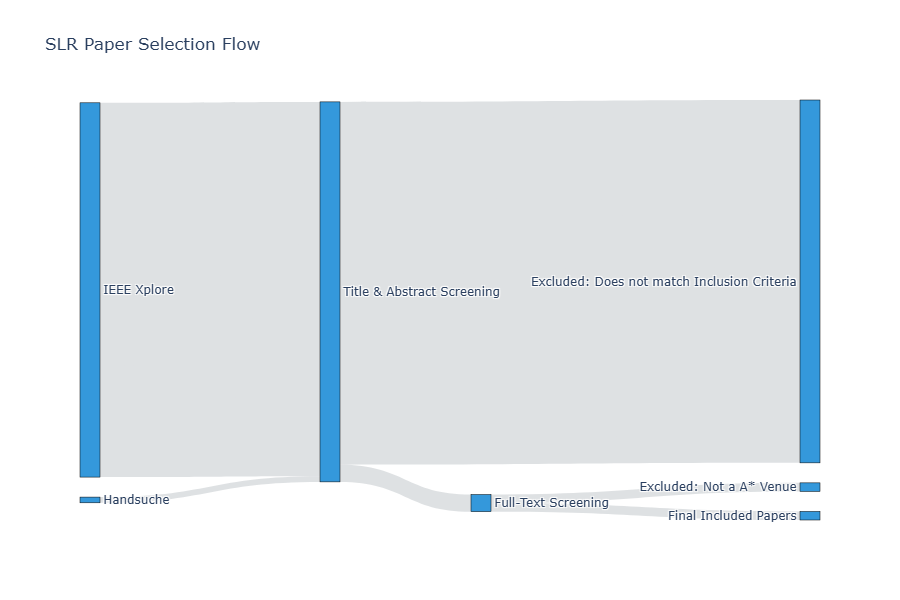
\includegraphics[width=1\linewidth]{images/selection_plot.png}
%     \caption{Auswahl der Arbeiten}
%     \label{fig:paper_selection}
% \end{figure}


\subsection{Überblick über das Korpus}

Aus den verbleibenden Arbeiten ergeben sich zunächst 5 verschiedene Benchmarks und 12 Arbeiten aus dem direkten Umfeld der Generierung von Quellcode. \todo{Ausbauen}

\section{Anforderungen als Eingabe}\label{ch:Anforderungen als Eingabe}

Diese Sektion befasst sich mit den spezifischen Eingabeartefakten, welche in den analysierten Arbeiten vorkommen. Das Format der Eingabe hat maßgeblichen Einfluss auf dessen Ausgabe. Schließlich lässt eine Formulierung in NL eine große Varianz and Detailgrad und technischem Inhalt zu, welcher wiederum Einfluß auf das Gesamtsystem hat. Ferner ergibt sich hier auch ein Einfluß auf die Autonomie des Systems.

\subsection{Kategorisierung der Eingabeformate}\label{ch:Kategorisierung der Eingabeformate}

Bevor die genauen Ergebnisse in Hinsicht auf die Eingaben vorliegen, lohnt es sich, eine formelle Kategorisierung von Eingabetypen vorzunehmen. Aus den analysierten Arbeiten lassen sich folgende distinkte Kategorien ableiten:

\begin{enumerate}
    \item \textbf{Unstruktuturierte Natürliche Sprache} \\ Einfache textuelle Beschreibungen, unformatierte Prompts
    \item \textbf{Strukturierte / Agile Artefakte} \\ Standartisierte Formate, z.B. User Stories
    \item \textbf{Formalisierte Anforderungen} \\ Ansätze bei denen initiale Anforderungen (aus einer anderen Kategorie) vor der tatsächlichen Eingabe (durch Verwendung von LLMs) formalisiert / diskutiert werden
    \item \textbf{Skizzen und erweiterte Repräsentatione}n \\ Eingaben die aus strukturierten Formatten bestehen, z.B. JSON
    \item \textbf{Test-basierte Eingaben} \\ Nutzung von Testfällen als Anforderungsspezifikation, ähnlich TDD\todo{oben erläutern oder hier oder weg lassen}
\end{enumerate}\todo{Hier noch Survey mit ins Spiel bringen falls dieser andere/bessere Befunde hat}

\subsection{Analyse der Eingabekategorien}\label{ch:Analyse der Eingabekategorien}

% \todo[inline]{Jede Kategorie als subsubsection, dann referenzieren mit den citations aus der Matrix und kurzer Erklärung was genau gemacht wurde, insofwern Abweichung der Definition oben besteht}

\subsubsection{Unstruktuturierte Natürliche Sprache}\label{ch:Analyse der Eingabekategorien:Unstruktuturierte Natürliche Sprache}



\todo[inline, color=blue]{ArchiLLM Analyse sucht noch einen Platz, hier passt es nicht gut hin.}
% \subsubsection{ArchiLLM}\label{ch:ArchiLLM}

% Die Forschungsfragen dieser Arbeit zielen vor allem auf die Präsentation von NL Anforderungen via User Stories ab. Wie bereits beschrieben, gibt es Stand heute praktisch keine Arbeiten, welche NL2Code via User Stories betrachten. Hier stellt \cite{calamoUserStoriesArchitectures2026} eine Ausnahme dar, weswegen diese Arbeit hier erwähnt wird.\todo{Formulierung Eröffnung anpassen}

% Die dabei vorgestellte Anwendung ''ArchiLLM'' schlägt einen neuen Ansatz vor, welcher bei der Entwicklung von Anwendungen die Zuverlässigkiet und Kohärenz erhöhnen soll. Zu diesem Zwecke stellt die Arbeit eine Pipeline vor:

% \begin{enumerate}
%     \item Extraktion von Microservices aus gegebenen User Stories
%     \item RAG Abfragen, gestützt durch Datensamlung zu Microservices Architecture
%     \item Generierung einer Architektur im JSON Format
%     \item Generierung einer Bare-Bones\todo{Begriff} Java Spring Boot Anwendung ohne implementierung von Anwendungs-Logik
% \end{enumerate}

% Trotz dieser [...] kann diese Arbeit leider im Rahmen dieser Arbeit nicht weiter betrachtet werden, da sie erhebliche Mengel mit sich bringt. Die Arbeit verifiziert ihre Ziele bzw. Aussagen nie gegen ihre Ergebnisse, es wird lediglich auf ein verlinktes Repository verwiesen. Die im Repository abgelegten Befunde und Auswertungen lassen sich allerdings nicht reproduzieren, da der gegebene Quellcode nicht ausführbar ist. Selbst nach Behebung von Fehler ergeben sich andere Zahlen als im Paper präsentiert. Die Methodik ist daher leider nicht nachvollziehbar und somit wird dieses Paper explizit nicht weiter verfolgt.

% In seinen Grundzügen ist die Arbeit allerdings trotzdem interessant für zukünftige Arbeiten: Sie präsentiert ein Datenmodell zur Evaluation von Ergebnissen, in denen User Stories von bestehenden studentischen Projekten gelabeled und jeweils bestimmten Microservices zugeordnet wurden. Dies eröffnet die Möglichkeit einer granularen Evaluation von generierten Microservices gegenüber der gegebenen Ground Truth.


\section{Ansätze zur Code-Generierung}\label{ch:Ansätze zur Code-Generierung}



\section{Evaluation in der Literatur}\label{ch:Benchmarks und Datensätze}

todo.

\subsection{Benchmarks}

\subsubsection{NL2Repo-Bench}

Bestehende Benchmarks evaluieren vor allem die Fähigkeiten von LLMs in der Generierung von lokalem Code oder auch die Reperatur von Code in geringeren Ausmaßen. Zur Evaluation von LLMs in einem größeren Kontext - der Exekution über größere Horizonte und näher an reellen Anwendungsbereichen aus der Softwareentiwcklung, präsentiert \cite{dingNL2RepoBenchLongHorizonRepository2026} den Benchmark $NL2Repo-Bench$. 

\todo[inline]{Vergleich nicht als paper/paper/paper sondern eher unter gemeinsamen Geischtspunknten. TODO: diese subsection entfernen und den Text in einen solchen Punk mit einarbeiten}


\section{Automatisierungsgrad}\label{ch:Automatisierungsgrad}



\section{Abgrenzung}\label{ch:Abgrenzung}\todo{Spezifizieren wie ich das am besten mache, siehe google doc letzte Konsultation (Notizen)}



\todo[inline,color=red]{AB HIER ALTER STAND ZUM RAUS KOPIEREN, DARÜBER NEUER STAND!}

% \todo[inline]{Einführung, Einordnung der Themengebiete im gröberem Kontext}

% \section{Anforderungsdokumente \& User-Stories}

% \todo[inline]{}

% \section{Datensätze zur Evaluation}

% \subsection{Evaluationsmetrkien}

% \subsection{Datensätze / Benchmarks}

% \section{Code Generierung}

% \todo[inline]{Zuerst Lösungs-übergreifende Erklärung, danach in die Details einzelner gewählter Lösungen}

% \subsubsection{Informationsbeschaffung wissenschaftlicher Literatur}

% Kernpunkt dieser Arbeit ist die Analyse von bestehenden Lösungen für \rqref{RQ1} und im erweiterten Rahmen auch \rqref{RQ2}. Neben den bereits angeführten Themenbereichen, sollen in dieser Sektion die tatsächlich existierenden Lösungsansätze für die Generierung von Quellcode aus Anforderungen analysiert werden. Um eine möglich umfangreiche Betrachtung durchführen zu können, muss demnach eine große Menge an wissenschaftlichen Arbeiten analysiert werden. In diesem Sinne bietet es sich an, eine ''Meta Analyse'', angelehnt an ein SLR (Structured Literature Review)\cite{kitchenhamGuidelinesPerformingSystematic2007} durchzuführen. 

% % Wie bereits angeführt soll im Ramen dieser Arbeit eine Analyse vorhandener Literatur stattfinden. Dabei ergeben sich Thematische Schwerpunkte welche der direkten Beanwortung der Forschungsfragen dienen:

% % \begin{itemize}
% %     \item Generierung von Quellcode aus Anforderungen
% %     \item Automatisierungsgrad von LLM (Multi-Agent) Systemen \textit{(für Quellcode Generierung)}
% % \end{itemize}

% % Weiterhin gibt es verschiedene Themenkomplexe welche durch ihre unmittelbare Nähe zu den Forschungsfragen \textit{oberflächlich} analysiert werden sollen:

% % \begin{itemize}
% %     \item Quellcode Generation durch Multi-Agent Systeme
% %     \item Generation von User Stories
% %     \item Generation von Tests (Unit, E2E, Integration, UAT)
% %     \item Evaluation von Ergebnissen (LLM-Judges, etc.)
% % \end{itemize}

% \subsubsection{Meta Analyse}

% % Hier soll zunächst die Outline für eine Meta Analyse definiert werden. Fokus der Analyse ist es, möglichst relevante wissenschaftliche Arbeiten zu sammeln und zu analysieren. Hinsichtlich des vorherigen Unter-Kapitels und in Betrachtung der Empfehlungen von \cite{kitchenhamGuidelinesPerformingSystematic2007} verfolge ich folgende Strategie:
% Das Ziel dieser Meta Analyse ist es, möglichst viele wissenschaftliche Arbeiten zum gegebenen Themenschwerpunkt zu sammeln und diese dann zu analysieren. Wie bereits erwähnt lehne ich mich hier an das Vorgehenes eines SLR\cite{kitchenhamGuidelinesPerformingSystematic2007} an und habe folgenden Durchführungsplan aufgestellt:

% \begin{enumerate}
%     \item Definition von Inklusions/Exklusions-Kriterien
%     \item Schlüsselwort Sammlung, daraus Queries definieren
%     \item Sammlung durch akademische Tools (IEEExplore, arXiv, etc.)
%     \item Bündelung und Sortierung von Ergebnissen
%     \item Filtern der Ergebnisse
% \end{enumerate}

% Nebene diesem groben, durch queries gestützen Prozess werden weiterhin auch händisch gefundene Arbeiten inkludiert. Für diese gelten allerdings die gleichen Kriterien.
% % Nach diesem Prozess sollten sich ca \textasciitilde 20 wissenschaftliche Arbeiten mit starker Relevanz ergeben.

% \subsubsection{Umsetzung Meta Analyse}

% \textbf{Strategie 1: SLR ähnliche Analyse via IEEExplore}

% \begin{enumerate}
%     \item Definition einer Query
%     \item Anwendung Inclusion Criteria (IC)
%     \item Anwendung Exclusion Criteria (EC)
%     \item Screening (Manual?=)
% \end{enumerate}

% \textbf{Query}

% Um möglichst viele Paper auf einmal zu gewinnen wird eine Query via IEEE Xplore ausgeführt. Hier wird bereits ein IC angewendet, da IEEE Xplore diese Funktionalität Diese sieht wie folgt aus:

% \begin{verbatim}
%     ("Large Language Model" OR LLM OR "Generative AI") 
%     AND ("User Story" OR Requirement) 
%     AND ("Code Generation" OR Autonomous OR "Multi-Agent")
% \end{verbatim}
% = 524 Arbeiten

% \textbf{Inclusion Criteria / Inklusionskriterien}

% \begin{enumerate}
%     \item Publikation zwischen 2023 und 2026
%     \item Arbeit behandelt die Transformation von natürlichsprachlich formulierten Anforderungen in Quellcode
%     \item Arbeit nutzt LLMs / Agentic Frameworks / Multi-Agent-Systeme
%     \item Arbeit evaluiert ihre Ergebnisse oder beschreibt die Architektur des Systems (am besten auch den Grad der Automatisierung)
% \end{enumerate}

% \begin{figure}
%     \centering
%     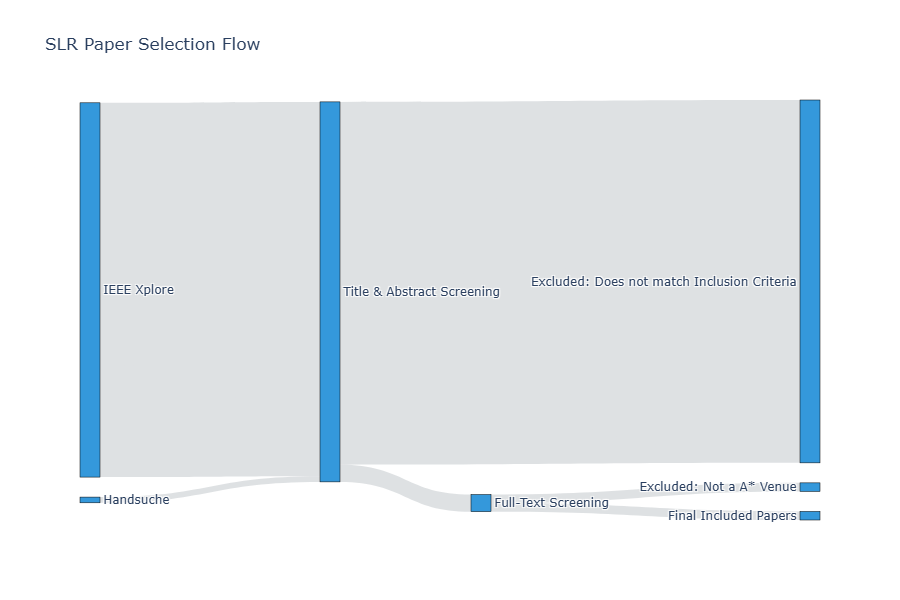
\includegraphics[width=1\linewidth]{images/selection_plot.png}
%     \caption{Auswahl der Arbeiten}
%     \label{fig:paper_selection}
% \end{figure}

% \section{Zusammenfassung}

% \begin{table}[t]
%     \todo[inline]{Summarize the properties, flaws, strengths, and weaknesses of all actually related publications here!}
%     \centering
%     \begin{tabular}{p{0.15\textwidth}|p{0.15\textwidth}|p{0.15\textwidth}|p{0.15\textwidth}|p{0.15\textwidth}}\hline\hline
%          & & & &  \\\hline\hline
%          & & & &  \\\hline
%          & & & &  \\\hline
%          & & & &  \\\hline
%          & & & &  \\\hline
%          & & & &  \\\hline
%          & & & &  \\\hline\hline
%     \end{tabular}
%     \caption{Overview of related work.}
%     \label{tab:placeholder}
% \end{table}

% #####################################################
% TODO: fragments that dont have a place yet
\todo[inline]{Text fragments I still need to sort under a section (more like subscetion)}
% #####################################################



\controlquestions{
Dieses Kapitel zeigt, welche wissenschaftlichen oder technischen Arbeiten es zu diesem Abschlussarbeitsthema bereits gibt, wie die Arbeit in diesen Kontext einzuordnen ist und welche Lücken geschlossen werden sollen.

\begin{itemize}
  \item {Einordnung des Themenumfelds}
  \begin{enumerate}
    \item Wurde beschrieben, welche Themenbereiche im Umfeld der eigenen Arbeit liegen (mit Begründung)? 
    \item Wurde das Umfeld der Arbeit qualifiziert und wissenschaftlich fundiert beleuchtet?
    \item Wird der aktuelle Forschungs- oder Entwicklungsstand zum Thema deutlich erkennbar gemacht?
  \end{enumerate}

  \item {Recherche und Auswahl der Literatur}
  \begin{enumerate}[resume]
    \item Wurden relevante Arbeiten systematisch und gezielt recherchiert (z.\,B.~über wissenschaftliche Datenbanken)?
    \item Deckt die Auswahl sowohl klassische (etablierte) als auch aktuelle Arbeiten ab?
    \item Sind die gewählten Arbeiten methodisch oder technisch mit der eigenen Arbeit vergleichbar?
    \item Wurden überwiegend wissenschaftliche Veröffentlichungen als Quellen angegeben?
    \item Wurden Quellen wie Wikipedia/Medium/Twitter/usw. explizit markiert und deren Vertrauenswürdigkeit diskutiert?
  \end{enumerate}

  \item {Inhaltliche Darstellung und Vergleich der Arbeiten}
  \begin{enumerate}[resume]
    \item Werden die Kernideen, Methoden und Ergebnisse der verwandten Arbeiten korrekt und prägnant dargestellt?
    \item Wurden die Stärken/Schwächen und idealerweise auch Chancen/Risiken (SWOT) der wichtigsten verwandten Arbeiten dargestellt?
    \item Wird deutlich, wie sich die verschiedenen Arbeiten inhaltlich oder methodisch voneinander unterscheiden?
    \item Welche Lücken existieren in den verwandten Arbeiten (liefert Rechtfertigung für die eigene Arbeit)? Wird transparent, was an bestehenden Arbeiten bereits gut funktioniert – und wo ihre Grenzen liegen?
    \item Werden die Arbeiten nicht einfach aufgezählt, sondern systematisch miteinander verglichen und diskutiert?
    \setcounter{lastenumcounter}{\value{enumi}}
  \end{enumerate}
\end{itemize}
}
\controlquestionscontinue{
\begin{itemize}
  \item {Ableitung und Abgrenzung der eigenen Arbeit}
  \begin{enumerate}[resume]\setcounter{enumi}{\value{lastenumcounter}}
    \item Wurde am Ende des Kapitels dargestellt, was der konkrete Fokus der eigenen Arbeit ist (mit Begründung)?
    \item Wurde klargestellt, was wiederverwendbar ist (als Konzept, Methode oder Tool)?
    \item Ergibt sich aus der Darstellung der verwandten Arbeiten ein logischer Übergang zur eigenen Problemstellung oder Motivation?
    \item Wurde im letzten Abschnitt eine Einordnung vorgenommen, welche Arbeiten die höchste Bedeutung für das eigene Thema haben?
    \item Wurde im letzten Abschnitt präzise hergeleitet, warum die eigene Arbeit gerechtfertigt ist, d.\,h. warum eine Forschungslücke existiert?
    \item Wird erläutert, wie die eigene Arbeit sich von den verwandten Arbeiten abgrenzt oder diese ergänzt?
    \item Wird klar, welchen wissenschaftlichen oder praktischen Mehrwert die eigene Arbeit im Vergleich bietet? Dies ist die Herleitung für die eigene konkrete Themenabgrenzung.
  \end{enumerate}

  \item {Zitierweise und Quellenqualität}
  \begin{enumerate}[resume]
    \item Sind alle Aussagen zu den verwandten Arbeiten korrekt belegt und mit fundierten Quellen versehen?
    \item Wird auf die begutachtete (peer-reviewed) Originalquellen und nicht nur auf Sekundärliteratur verwiesen?
  \end{enumerate}

\end{itemize}

}

\chapter{Anforderungen und Konzept}\label{ch:Anforderungen und Konzept}

[...]. Fundamental für diese Arbeit ist es, bestehende Arbeiten aus Kapitel \ref{ch:Verwandte Arbeiten} auf ihre tatsächliche Fähigkeiten zu vergleichen. Um solche Vergleichswerte zu erhalten, bedarf es eigener Experimente, in welchen Code-Generierungs Anwendungen unter gleichbleibenden Bedienungen gegen bestehende Benchmarks ausgeführt werden. In diesem Kapitel sollen die Anforderungen und ds Konhept an diese Experimente erläutert werden.\todo{Rewrite I think, das greift etwas vor}

\section{Anforderungen}\label{ch:Anforderungen}

Um die Forschungsfrage \rqref{RQ1} zu beantworten, wird ein empirischer Vergleich benötigt. Ein solcher Vergleich lässt sich aus den gegebenen Arbeiten allerdings nur schwer ableiten, da die Rahmenbedienungen für die gegebenen Lösungen und deren Evaluation stets unterschiedlich sind. Wir haben hier bereits festgestellt dass:

\begin{itemize}
    \item LLM Modelle
    \item Hyperparameter
    \item Benchmarks und deren Umgebungen
\end{itemize}

in praktisch jeder Arbeit Unterschiede aufweisen. Insofern bedarf es einen eigenen, kontrollierten Versuchsaufbau, mit dem gewährleistet werden kann, dass diese Faktoren konsistent bleiben. Aus dieser Notwendigkeit soll in diesem Kapitel das Konzept für einen solche Aufbau präsentiert werden.

Am Rande gilt es hier zu erwähnen, dass für die Beantwortung von \rqref{RQ2} kein Versuchsaufbau genutzt wird.

\subsection{Funktionale Anforderungen}\label{ch:Funktionale Anforderungen}

Nun gilt es die Anforderungen an eine solche Anwendung zu spezifizieren, damit wir diese in einer späteren Implementierung nachvollziehen können. Es ergeben sich folgende funktionale Anforderungen:

\textbf{Invarianz}\label{req:FA1} \\ Es muss möglich sein, beliebige Lösungsansätze gegen beliebige Benchmarks zu prüfen (bzw. auszuführen).

\textbf{Konfiguration}\label{req:FA2} \\ Eine einheitliche Schnittstelle existiert, die es ermöglicht Modelle, Hyperparameter sowie Lösungsansätze frei zu konfigurieren.

\textbf{Isolation}\label{req:FA3} \\ Die Ausführung von Lösungsansätzen und Benchmarks muss in isolierten Umgebungen stattfinden.

\textbf{Bewertung}\label{req:FA4} \\ Die Bewertung des generierten Codes eines Lösungsansatzes erfolgt ausschließlich durch den gegebenen Benchmark.\todo{Name finden}

\textbf{Protokollierung}\label{req:FA5} \\ Für einzelne Durchläufe werden alle Parameter, Versionen sowie ausgegebene Dateien protokolliert. 

\todo[inline]{Ist wiederholbarkeit evtl. eine Anforderung? Wie läuft das mit Temperature?}

\todo[inline, color=red]{Evtl. die Namen mit ID's versehen, FA1, FA2 und dann NFA1 usw!}

\subsection{Nicht-funktionale Anforderungen}\label{ch:Nich-Funktionale Anforderungen}

Neben den bereits genannten funktionalen Anforderungen, ergeben sich weiterhin auch Nicht-funktionale Anforderungen:

\begin{enumerate}
    \item Generierter Code muss unabhängig und isoliert von seiner Umgebung laufen können. Das selbe gilt für die Bewertung.
    \item Der laufende Benchmark bewertet die Ergebnisse einer laufenden Code-Generierungsanwendung. Die Bewertung wird einzig und allein vom Benchmark definiert.
    \item Alle Code-Generierungsanwendungen müssen austauschbar sein. Dafür dürfen weder der Benchmark noch andere funktionale Aspekte der Anwendung verändert werden.
    \item Jeder Durchlauf eines Experiments muss vollständig nachvollziehbar sein. Versionen, Modelle und Parameter müssen auch nach Durchführung ersichtlich sein.
\end{enumerate}
\todo[inline]{Auch wie funktionale Anforderungen labeln und mit Obernahmen versehen damit die dann in dre Umsetzung referenziert werden können!}

\subsection{Rahmenbedienungen \& Abgrenzung}\label{ch:Rahmenbedienungen_Abgrenzung}

\todo[inline]{Sind externe Abhängigkeiten oder Rahmenbedingungen (z. B.
Plattformen, Zielgruppen, Datenquellen) eindeutig und nachvollziehbar
dargestellt?}

Neben den formulierten Anforderungen muss der Umfang der Anwendung abgegrenzt werden. Auf Grund des Budgets für diese Arbeit ist es nicht möglich massive Testreihen durchzuführen welche z.B. die Evaluationsmetrken $pass@10$ oder gar $pass@100$ abdecken können. Weiterhin gibt es keinen Benchmark welcher User-Stories als Eingabeartefakte bereit stellt. Daher wird hier klar festgelegt dass ein solcher Benchmark nicht Teil der Anforderungen oder der Konzeption sein kann.

Weiterhin ist im Sinne der Integrität zu erwähnen, dass die zu testenden Lösungsansätze in ihrer internen Logik nicht verändert werden dürfen. Lediglich nicht-Logikbasierte Eingriffe (z.B. eine Modifikation, die das Einstellen aller Hyperparameter innerhalb eines LLMs Zugriff ermöglicht) sind erlaubt, da diese für eine uniforme Durchführbarkeit vonnöten sind. Eine Außnahme gilt in diesem Kontext für die Nutzung von selbst etablierten Verfahren, da die Logik hier grundlegend erst geschaffen werden muss und nicht von aussenstehenden Arbeiten stammt.

Eine weitere Abgrenzung gilt den Zielsprachen des generierten Codes. Dieser kann nicht frei gewählt werden, da er direkt vom Benchmark und dessen Evaluation abhängig ist.
\todo[inline]{Falls SWE-Pro (oder verified?) dann evtl erwähnen dass es hier mehr als Python gibt. Ansonsten einfach sagen dass es halt nur Python ist, nicht mehr. Das könnte man auch am Ende nochmal auffassen, da es hier bereits angesprochen wurde.}

\section{Konzept}\label{ch:Konzept}

In dieser Sektion soll das Konzept des Versuchsaufbaus erläutert werden. 

\subsection{Untersuchungsdesign}\label{ch:Untersuchungsdesign}

Zu Grunde liegt dass Problem der Vergleichbarkeit. Praktisch alle referenzierten Arbeiten hab eine vielzahl an Parametern, mögen diese spezifische Hyperparameter oder globalere Parameter wie Modelle oder sogar Benchmarks sein. Dies macht es fundamental nicht möglich einen klaren Vergleich zu ziehen, denn für diesen dürfte sich wenn möglich nur ein Parameter ändern, nämlich der Lösungsansatz zur Code-Generierung.

Aus diesem Grund verläuft die Untersuchung in dieser Arbeit wie folgt:

\begin{enumerate}
    \item \textbf{Vergleich Paper zu lokaler Arbeit} \\ Zunächst muss etabliert werden, ob die lokale Lösung dieser Arbeit die selben Ergebnisse erzeugen kann wie die aus dem Ausgangs-Paper. Paper beschreiben bereits genutzte Modelle, Benchmarks und Hyperparameter, diese können daher übernommen werden und im lokalen Versuchsaufbau getestet werden. Falls dabei Diskrepanzen gefunden werden, müssen diese aufgenommen werden um später in der Interpretation der Ergebnisse mit einzuwirken.
    \item \textbf{Vergleich der Lösungsansätze} \\ Nachdem festgestellt wurde wie die Lösungsanästze im Vergleich zu den original beschriebenen Werten agieren, sollen diese hier untereinander verglichen werden. Ziel dabei ist es wie bereits beschrieben möglichst alle Parameter in jedem Durchlauf gleich zu lassen, so dass alle Lösungsansätze die gleichen Voraussetzungen haben.
\end{enumerate}

Vor allem für den zweiten Schritt, den \textit{Vergleich der Lösungsansätze}, mangelt es allerdings an Referenzwerten. Neben den Lösungsansätzen, die in dieser Arbeit für eine weitere Betrachtung ausgewählt werden, sollen zwei weitere Werte mit aufgenommen werden:

\begin{enumerate}
    \item \textbf{Single-Shot Baseline} \\ Mit diesem Verfahren soll eine Baseline etabliert werden, die praktisch eine Untergrenze definiert. Sie beantwortet die Frage, was das Modell mit seinen Hyperparametern ohne ein Gerüst liefern kann. Spezifisch soll hier die Anwendung von Zero-Shot Prompting (siehe \ref{ch:prompting:early}) stattfinden. Weiterhin handelt es sich den Namen nach entsprechend um einen single-shot, das bedeutet nur ein Input und ein Output sind erlaubt. Die Awendung ist damit so einfach wie möglich gestrickt um eine wahre Baseline zu etablieren.
    \item \textbf{Agentisches Verfahren} \\ Die betrachteten Arbeiten stellen vermehrt die These\todo{Vorsicht! Prüfen!} auf, dass sie bessere Ergebnisse als generische Verfahren liefern. Zu diesem Zweck soll ein Agenten-System ohne spezifischen Fokus auf Quellcode Generierung genutzt werden um diese Hypothese zu überprüfen.
\end{enumerate}

Mit diesen Komponenten ist es möglich genau zu überprüfen wie akkurat die präsentierten Lösungen tatsächlich sind. 

\subsection{Operationalisierung}

\todo[inline]{Erklären wie die Forschungsfragen messbar gemacht werden --> pass rate / pass@k}

Ebenfalls muss hier eine Abgrenzung hinsichtlich der Forschungsfrage \rqref{RQ1} gemacht werden. Diese betrachtet neben Quellcode auch zugehörigen Text, eine Anforderung die keiner der etablierten Benchmarks überprüft oder bewertet. Eine Bewertung dieser Anforderung ist daher im Rahmen dieser Arbeit nicht möglich.\todo{Oder ich kürze das einfach aus der Forschungsfrage? Kann ich eh nicht machen....}

\subsection{Kontrollierte und variable Parameter}

Das Ziel der Experimente ist der Vergleich verschiedener Lösungsansätze. Ein solcher Vergleich unterliegt der Bedienung, dass Parameter zwischen den Testdurchläufen nicht verschieden modifiziert werden, da die Auswertung der Ergebnisse sonst schlichtweg unmöglich ist. Würden sich zwischen den Durchläufen mehr als 1 Parameter ändern, so ist es danach folglich nicht möglich die Resultate gegenüber zu stellen, da sich die Ursache nur schwer begründen lässt.

Aus diesem Grund werden hier die Parameter genannt welche durch die Anwendung kontrolliert werden, welche variabel sind und welche Parameter nicht kontrollierbar sind.

\subsubsection{Kontrollierte Parameter}

\begin{itemize}
    \item Modell (LLM)
    \item Endpunkt des Modells
    \item Inferenzparameter
    \item Benchmark und dessen Version
    \item Auswahl an Aufgaben aus einem Benchmark
    \item Ausführungsumgebung
    \item Anzahl der Durchläufe
\end{itemize}

\subsubsection{Variable Parameter}

Der einzige bewusste variable Parameter ist der Lösungsansatz. Da das Ziel ist diese gegeneinander zu testen, muss dieser Parameter variabel sein.

\todo[inline]{Was hier noch fehlt - es gibt 2 Modus Operandi. 1. Es ändert sich nur das Codegen tool zum Vergleichen und 2. Der Versuchsaufbau des zugrunde liegenden Papers wird durchgeführt.}

\subsubsection{Nicht kontrollierte Parameter}

\begin{itemize}
    \item Nichtderminismus der Inferenz\todo{evtl in Ch.2 erläutern}
    \item Anbieterseitige Modelländerungen
    \item Rate Limits der Anbieterplatform
    \item Netzwerkeffekte
\end{itemize}

\subsection{Architektur des Aufbaus}

Diese Sektion behandelt die Architektur, welche aus den Anforderungen abgeleitet wurde. Der Entwurf der Architektur wird mittels PlantUML dargestellt und ist zunächst ein roher Entwurf, zu betrachten in \ref{fig:rough_architecture}.

\begin{figure}[H]
    \centering
    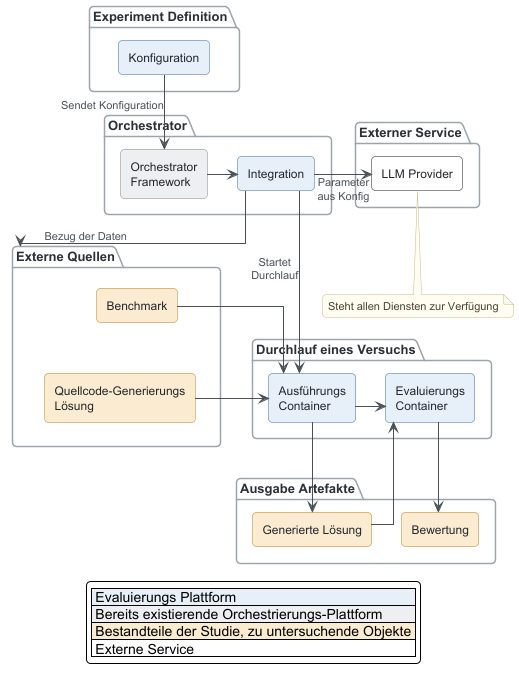
\includegraphics[width=1\linewidth]{images/rough_architecture.png}
    \caption{Architektur der Evaluierungs Plattform}
    \label{fig:rough_architecture}
\end{figure}

Zentraler Bedeutung ist hier zunächst die eigene Integration, welche Verantwortlich für die Nutzung von Quellcodelösung und Benchmark ist. Durch sie muss dem etablierten Orchestrator Framework ermöglicht werden dedizierte Container für die Durchführung von Experimenten zu erstellen. Diese Container führen dann die Generierung und die Evaluierung von Lösungen aus.

Sowohl die generierte Lösung als auch die Bewertung des Benchmarks müssen außgegeben werden. Um den Anforderungen gerecht zu werden, müssen die ausgegebenen Artefakte aber auch die Konfiguration des Experiments und alle relevanten Parameter beinhalten, denn nur so ist es möglich diesen Prozess später nachzuverfolgen.

\subsection{Annahmen und Alternativen (?)}

\todo[inline]{Bei Alternativen wirklich überlegen ob das hier Halt hat, ist nur erstmal eine Idee in Hinsicht auf Kontrollfrage 16. Deckt sich evtl schon etwas mit subsection zu Abgrenzung.}

\controlquestions{
Für dieses Kapitel in einer Abschlussarbeit ist es wichtig, dass sowohl die Ziele und Anforderungen an die Lösung sauber hergeleitet als auch ein durchdachtes Konzept zur Erfüllung dieser Anforderungen präsentiert.
Dieses Kapitel baut in der Regel direkt auf der Analyse des Problems oder des Status quo auf und legt die Grundlage für die spätere Umsetzung.
\begin{enumerate}
    \item Wurden die Anforderungen aus den Forschungsfragen (siehe Kapitel \ref{ch:Motivation und Problemdefinition}) hergeleitet?
    \item Ist der Zusammenhang zwischen Anforderungen und übergeordneten Zielen/Forschungsfragen nachvollziehbar?    
    \item Gibt es eine nachvollziehbare Verbindung zu den Erkenntnissen aus der Analyse der verwandten Arbeiten (vgl.~Kapitel \ref{ch:Verwandte Arbeiten})?
    \item Sind funktionale Anforderungen angemessen berücksichtigt sowie eindeutig und vollständig formuliert?
    \item Sind nicht-funktionale Anforderungen eindeutig und vollständig formuliert?
    \item Sind die Anforderungen überprüfbar/testbar formuliert?
    \item Sind externe Abhängigkeiten oder Rahmenbedingungen (z.\,B. Plattformen, Zielgruppen, Datenquellen) eindeutig und nachvollziehbar dargestellt?
    \item Ist klar, welches Ziel das Konzept verfolgt?
    \item Ist das vorgeschlagene Konzept logisch und konsistent aufgebaut?
    \item Ist die Systemarchitektur bzw. das technische Design verständlich und nachvollziehbar beschrieben?
    \item Wurden Entscheidungen aus den Anforderungen oder aus der Literatur (vgl.~Kapitel \ref{ch:Verwandte Arbeiten}) hergeleitet?
    \item Wurden Annahmen getroffen oder Einschränkungen akzeptiert – und sind diese offengelegt und diskutiert?
    \item Ist ersichtlich, auf welchen Annahmen das Konzept basiert?
    \item Wird erklärt, wie das Konzept die zuvor definierten Anforderungen erfüllt?
    \item Gibt es Abbildungen (z.\,B.~UML-Diagramme, Systemübersichten, Prozessmodelle), die die Umsetzung visualisieren?
    \item Wurden Alternativen zum Konzept dargestellt, die in Betracht gezogen oder bewusst ausgeschlossen wurden?
    \item Ist das Konzept unabhängig von der konkreten Umsetzung (also ohne den Quellcode) verständlich?
    \item Ist das Konzept so (nachhaltig) formuliert, dass es auch anders umgesetzt/implementiert werden könnte?
\end{enumerate}
}
\chapter{Implementierung}\label{ch:Implementierung}

Aus den bis hier beschriebenen Anforderungen für die Ausführung der Experimente ergibt sich die Notwendigkeit einer eigenen Software Lösung. Existierende Lösungsansätze müssen gegen verschiedene Benchmarks ausgeführt und evaluiert werden - geleitet von einer zentralen Platform, einen Orchestrator. Zu diesem Zweck habe ich\todo{"ich"? wie formuliert man das?} das Tool ''EvaluationPlatform'' gebaut. Dieses ist offen zugänglich und kann auf GitHub\footnote{https://github.com/Tim-Dietrich/EvaluationPlatform} gefunden werden. Dieses Kapitel beschreibt im weiteren die zugrunde liegenden Entscheidungen, die beim entwickeln der Anwendung getroffen wurden und wie diese implementiert wurde. 

\section{Wahl des Tech-Stacks}\label{ch:Wahl des Tech-Stacks}

% Diese Sektion beschreibt die Anwendung, welche gebaut wurde um die Fragen \rqref{RQ1} und \rqref{RQ2} transparent und möglichst gerecht beantworten zu können. Dabei wird erklärt wie diese Anwendung sturkturiert wurde und welche Entscheidungen dafür getroffen wurden.

\todo[inline]{Info: ''Ziel der Anwendung'' gehört hier nicht hin, das ist Konzept/Anforderungen. Die Obligationen wurden nach NFA verschoben.}
% \subsubsection{Ziel der Anwendung}\label{ch:Ziel der Anwendung}

% Wie bereits in \todo{ref to Oben, Struktur Idee etc.} beschrieben wurde, sollen in dieser Arbeit bestehende Lösungsansätze verglichen werden. Dies passiert wie in \todo{ref to Benchmarks} beschrieben via Benchmarks, welche genutzt werden um jeden Lösungsansatz unter gleichen Bedienungen zu testen. Zu diesem Zweck bedarf es einer Anwendung welche diesen Ablauf gewährleisten kann. Diese Platform unterliegt im Grunde 4 verschiedenen Obligationen:

% \begin{enumerate}
%     \item Generierter Code muss unabhängig und isoliert von seiner Umgebung laufen können. Das selbe gillt für das Grading
%     \item Der laufende Benchmark bewertet die Ergebnisse einer laufenden Code-Generierungsanwendung. Die Bewertung wird einzig und allein vom Benchmark definiert.
%     \item Alle Code-Generierungsanwendungen müssen austauschbar sein. Dafür dürfen weder der Benchmark noch andere funktionale Aspekte der Anwendung verändert werden.
%     \item Jeder Durchlauf eines Experiments muss vollständig nachvollziehbar sein. Versionen, Modelle und Parameter müssen auch nach durchführung ersichtlich sein.
% \end{enumerate}

% \todo[inline]{Erklären welche Parameter wir fest halten und welche evtl. variabel sein könne, siehe Prof. Both Konsultation \#6}

% Der Umfang dieser Anwendung wird bewusst schmal gehalten. Zweck ist lediglich das orchestrieren von Experimenten unter den bereits genannten Gesichtspunkten. Damit existiert eine klare Abgrenzung zu anderen Platformen, wie z.B. ''Bestenlisten'' oder ''Agent-Frameworks''.

% \subsubsection{Wahl eines Frameworks}

Der Umfang dieser Arbeit ist lediglich die Evaluation bestehender Lösungen. Somit ist es ziehlführend, bereits existierende Lösungen / Frameworks für die Nutzung eines Orchestrators einzubinden, anstatt diesen selbst zu kreieren. Eine solche bestehende Plattform erlaubt es den Fokus dieser Arbeit auf die Evaluation von existierenden Lösungen zu legen, anstatt zuerst selbst eine Plattform erstellen zu müssen.

Um die Wahl einer Orchestrierungsplatform zu begründen wurde ein explorativer Machbarkeitsversuch durchgeführt. Dieser Bestand aus dem Ziel, die Plattform aufzusetzen und einen einfachen Task zu starten. Der Task war hier lediglich das generieren eines lauffähigen Taschenrechners mit minimalen Funktionen. 

Es ist relevant hier zu erwähnen dass die Evaluation pur explorativ war und nicht systematischer Natur. Weiterhin wurde diese Exploration durch die Nutzung von LLM basierten Agenten umgesetzt. Die Wahl der zu nutzenden Plattform ist daher eher als Mittel zum Zweck zu sehen, nicht als Ergebnis dieser Arbeit.

Die Evaluation der Plattformen erfolgte gegenüber den Anforderungen, welche in den Sektionen \ref{ch:Funktionale Anforderungen} sowie \ref{ch:Nich-Funktionale Anforderungen} definiert wurden. Die betrachteten Plattformen wurden durch händische Suche gefunden.

Es ergaben sich daraus folgende Evaluierungen:

\begin{enumerate}
    \item \textbf{Eigene Plattform} \\ Wie bereits beschrieben, ist das Entwickeln einer eigenen Plattform nicht im Rahmen dieser Arbeit. Der Aufwand gegenüber allen Anforderungen wäre eine komplette Selbst-Entwicklung, was hier nicht tragfähig ist. Somit scheidet diese Option faktisch aus.
    \item \textbf{Benchmark-spezifische Skripte} \\ Die betrachteten Benchmarks (z.B. NL2Repo-Bench, SWE-Pro) kommen jeweils mit eigenen Skripten, um deren Ausführung zu ermöglichen. Dies funktioniert prinzipiell, erfordert aber ähnlich zur eigenen Plattform maßgeblichen Entwicklungsaufwand. Ferner ist durch die unterschiedlichen Implementierungen keine Vergleichbarkeit unter den verschiedenen Benchmarks gegeben. Aus diesem Grund wurde diese Option nicht weiter evaluiert.
    \item \textbf{Inspect AI} \\ TODO nachtragen
    \item \textbf{Harbor} \\ TODO nachtragen
\end{enumerate}

Nach Ablauf dieser Evaluation wurde sich für Harbor als zugrunde liegende Plattform entschieden. Neben der relativ einfachen Implementierung, deckt dieses Framework auch am besten die gegebenen Anforderungen ab. Wie bereits erwähnt, ist allerdings auch Harbor nicht in der Lage, alle Anforderungen ohne einen eigenen Entwicklungsaufwand zu erfüllen. 

\todo[inline, color=red]{Anforderungs-ID's sind doch notwendig! nachholen!}

\section{Architektur der Evaluierungsplatform}\label{ch:Architektur der Evaluierungsplatform}

Diese Sektion stellt die tatsächliche Implementierung der Evaluierungsplattform dar. Zum besseren Verständniss wurde die Architektur in 2 Einzelteile aufgeteilt:

\begin{enumerate}
    \item Das initiale Setup für den Orchestrator
    \item Die Architektur einer tatsächlichen Durchführung
\end{enumerate}

Hierbei gilt zu unterscheiden woher die verschiedenen Komponenten stammen. Zu diesem Zweck dient zunächst eine farbliche Legende, diese ist in der Figur \ref{fig:legend} zu erkennen.

\begin{figure}[H]
    \centering
    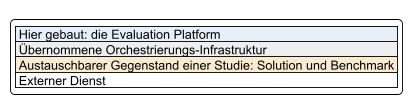
\includegraphics[width=0.75\linewidth]{evaluation_legend.png}
    \caption{Enter Caption}
    \label{fig:legend}
\end{figure}

Wir bereits in den Anforderungen beschrieben\todo{ref zur ID}, benötigt die Evaluierung zwingend eine feste einheitliche Definition aller Experimente. Bevor ein Durchlauf auf den tatsächlichen Integrator (hier Harbor) zugreift, muss also die Definition des Experimentes validiert und aufgelöst werden. Dieser Prozess ist in Figur \ref{fig:setup} zu sehen.

\begin{figure}[H]
    \centering
    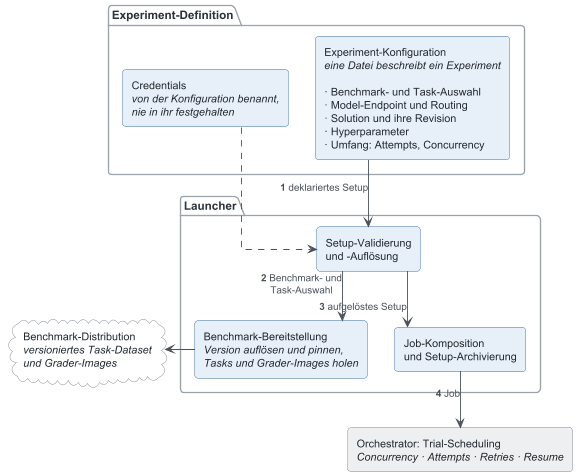
\includegraphics[width=1\linewidth]{evaluation_setup.png}
    \caption{Enter Caption}
    \label{fig:setup}
\end{figure}

\todo[inline, color=red]{WARNUNG: TEXT AUS ALTEM KAPITEL ÜBERNOMMEN; FÜR DIESE SEKTION ANPASSEN!}

Mit Harbor haben wir ein bestehendes Framework welches die Integration von verschiedenen Benchmarks durch seine eigene Dataset registry erlaubt. Währe das Ziel unserer Experimente die Evaluation von nativen Agenten/LLM-Integrationen würde dies für die weitere Durchführung genügen. Allerdings ergeben sich im Kontext dieser Arbeit 2 notwendige Änderungen:

\begin{enumerate}
    \item Das Ziel ist das Testen von Code-Generierungsanwendungen. Diese arbeiten nicht nach genormten Verfahren, jede Lösung ist individuell.
    \item Nicht \textit{alle} Benchmarks können nativ durch Harbor abgedeckt werden. Insbesondere NL2RepoBench\todo{cite} benötigt eine Anpassung, da den Entwicklern ein Fehler beim aufsetzen des Docker Images unterlaufen ist.
\end{enumerate}

Um diese Probleme zu beheben werden für alle integrierten Code-Generierungsanwendungen Integrationen geschrieben. Weiterhin existiert eine besondere Integration für NL2RepoBench, die dafür sorgt dass das benötigte Image über eine öffentlich zugängliche Platform bezogen wird. Die Integration für die einzelnen Code-Generierungsanwendungen wird in den jeweiligen Kapitel beschrieben um eine höhrere Transparenz zu gewährleisten. Fundamental dabei ist es, dass die Logik besagter Lösungen \textbf{nicht} angepasst wurde. Gemachte Modifikationen dieser Repositories zielen lediglich auf eine mögliche Integration ab, z.B. die Integration von Umgebungsvariablen via DotEnv\todo{evtl cite} Dateien.

\todo[inline]{Schlussendliche Erklärung der gewählten Architektur}

\begin{figure}[H]
    \centering
    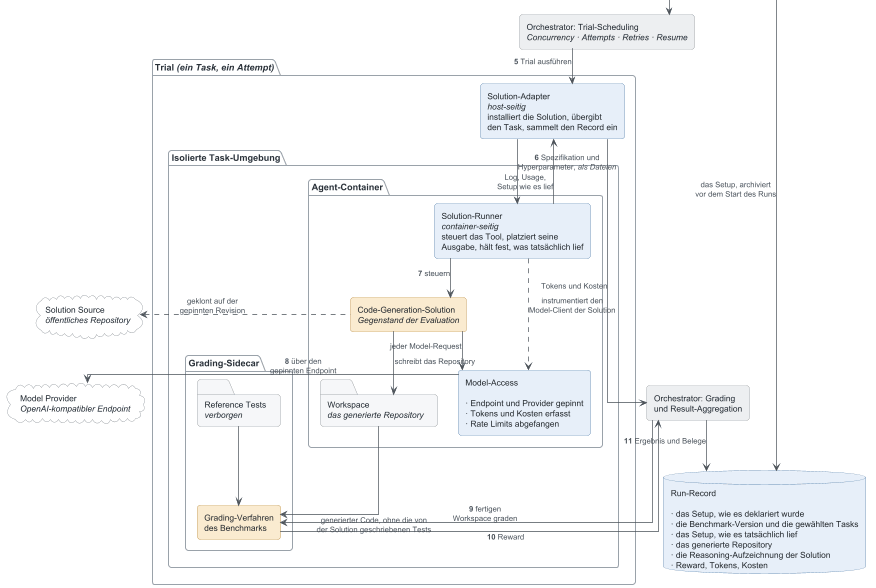
\includegraphics[width=1\linewidth]{evaluation_run.png}
    \caption{TODO: das passt von der größe nicht. Irgendwie was anderes ausdenken.}
    \label{fig:full_run}
\end{figure}

\section{Integration der Code-Generierungsanwendungen}\label{ch:Integration der Code-Generierungsanwendungen}

Wie bereits beschrieben lassen sich bestehende Code-Generierungsanwendungen nicht ohne weiteres in die Anwendung integrieren. Zwar haben einzelne Anwendungen wie \cite{dongSelfCollaborationCodeGeneration2024} bereits funktionierende Integrationen für Benchmarks, so ist es mit diesen aber nicht möglich eine uniforme Durchführung von Experimenten zu gewährleisten.

Demnach bedarf es für jede Anwendung einer Integration in den Harbor Workflow. Zuerst können damit folgende Kriterien sichergestellt werden:

\begin{enumerate}
    \item Freie Modelauswahl 
    \item Hyperparameter sind konfigurierbar
    \item Anwendungs-spezifische Parameter sind konfigurierbar
\end{enumerate}

Die Konfiguration dieser Werte erfolgt in der Evaluierungs-Platform und wird lediglich an die einzelnen Code-Generierungsanwendungen weitergereicht. Dabei unterstützen die einzelnen Konfigurationsdateien alle einzigartigen Parameter. Im folgenden ergeben sich daraus folgende Integrationen:

\todo[inline]{Integrationen für die einzelnen Anwendungen auf-listen mit ihren spezifischen Anforderungen.}

\subsection{Code-Team}

bla bla und so weiter mit subsections

\section{Implementierung der Referenz-Ansätze}

Die Sektion \ref{ch:Untersuchungsdesign} formuliert neben der Untersuchung bestehender Arbeiten auch die Inklusion von Referenzwerten durch zwei weitere Systeme (Single-Shot Basline \& Agentisches Verfahren). Im Gegensatz zu der Sektion \ref{ch:Integration der Code-Generierungsanwendungen} handelt es sich bei diesen Ansätzen nur bedingt um Integrationen, weswegen diese hier getrennt betrachtat werden.

\subsection{Single-Shot Baseline}\label{ch:Impl:Single-Shot Baseline}

Als Baseline im Vergleich dieser Arbeit dient ein Single-Shot-Ansatz. Die Implementierung dieses Ansatzes ist wie folgt geschehen:

\begin{enumerate}
    \item \textbf{Setup} \\ Initial werden analog zu anderen Ansätzen die Parameter der gegebenen Konfiguration bezogen.
    \item \textbf{Prompt-Erstellung} \\ Nach dem initialen Setup erfolgt die Erstellung des fertigen Prompts. Das Design dieses Prompts ist wichtig, denn er darf keine Lösungsstrategie angeben. Der hier genutzte Prompt \autoref{lst:prompt-singleshot} erklärt lediglich die vom Parser erwartete Ausgabestruktur, ohne die eine weitere Auswertung durch Harbor nicht möglich wäre. Die Anforderungen definieren weiterhin ''Zero-Shot'', weshalb keine Beispiele an den Prompt angehangen werden.
    \item \textbf{Ausführung} \\ Die vollständige Beschreibung der Aufgabe sowie der gegebene Prompt werden an das konfigurierte Modell übergeben.
    \item \textbf{Parsing} \\ Nach Antwort des Modells werden die Ergebnisse geparsed. Sollte die Antwort der erwarteten Struktur entsprechen, wird sie in einzelne Datein aufgeteilt und für die Evaluation im \texttt{workspace} Verzeichnis abgelegt.
\end{enumerate}

Nach diesem Ablauf erfolgt die gewohnte Evaluierung des Benchmarks, welcher durch das Harbor Framework orchestriert wird.

\subsection{Agentisches Verfahren}\label{ch:Impl:Agentisches Verfahren}

Das zweite Verfahren, welches als Refernz dient, ist das agentische Verfahren. Bei der Implementierung wurde keine explorative Suche oder eine Studie in betracht gezogen um ein Agenten-System auszuwählen. Da die Schaffung eigener Systeme prinzipiell nicht im Rahmen dieser Arbeit ist, wurde hier das bereits von Harbor bereitgestellte Agenten-System Terminus-2 \cite{Terminus2} gewählt.

Durch die bereits existierend Integration in den Harbor Workflow bedarf es hier keiner klassischen Integration wie bei bereits genannten Verfahren, allerdings mussten trotzdem kleine Anpassungen erfolgen:

\begin{enumerate}
    \item Die Vermittlung von Credentials erfolgt im Projekt durch eine speziell dafür geschaffene Überbrückung.
    \item Hyperparameter sind prinzipiell gleich; allerdings stellt Terminus-2 als Agenten-System einen extra Parameter \texttt{max\_turns} bereit, welcher hier gesondert konfiguriert werden muss. Dieser Parameter definiert die maximale Menge an Schritten des Agenten, was später für die Vergleichbarkeit wichtig wird.
\end{enumerate}

Das Verhalten des Agenten ist in dieser Implementierung nicht weiter beeinflußt.

\subsubsection{Terminus-2}

Ferner soll der von Harbor bereitgestellte Agent Terminus-2 hier kurz erklärt werden. Das Augenmerk liegt auf dessen Fähigkeiten und Eigenschaften, entnommen von \cite{Terminus2}:

\begin{itemize}
    \item Terminus-2 ist eine Implementiernug eines Agenten, gedacht zur Evlauation von LLMs bei deren Arbeit in Kommandozeilen Umgebungen.
    \item Es nutzt einen selbst betietelten ''single-tool approach'', durch welchen es in der Lage ist Tastenanschläge zu simulieren, Umgebungen zu navigieren, durch Output zu scrollen, Shells zu starten und mit Kommandozeilen-basierten Anwendungen zu interagieren.
    \item Die Ausführung der Logik läuft in einem sepparatem Python Prozess, welcher durch eine Docker-basierte Ausführung sicher und isoliert arbeitet. Der Agent hat somit nur Zugriff auf gegebene Aufgaben.
    \item Terminus-2 agiert vollständig Autonom und nimmt keine weiteren User-Inputs entgegen.
\end{itemize}

Analog zum Single-Shot-Ansatz erhält der Agent lediglich die Anweisung der Aufgabe als Input. Es werden keinerlei weitere Informationen zum Lösen einer Aufgabe übermittelt, welche die Ergebnisse nachhaltig fälschen würden. 

\section{Integration der Benchmarks}\label{ch:Integration der Benchmarks}

Die Integration von Benchmarks ist durch das Harbor Framework trivial. Benchmarks werden nativ unterstützt und können über die Harbor Registry ausgeführt werden.

\todo[inline]{Am Ende nochmal gegen prüfen ob das so korrekt ist.}

\subsection{Integration für NL2Repo-Bench}

Der einzige Benchmark der einer Integration bedarf ist NL2Repo-Bench. Dieser ist zwar ebenfalls in der Harbor Registry verfügbar, lässt sich allerdings nicht ausführen. Die Ursache für diesen Fehler liegt weder in Harbor noch der Integration. Der Benchmark ist sowohl auf GitHub\cite{GitHubMultimodalartprojectionNL2RepoBench2026}, als auch Harbor\cite{HarborHub} verfügbar.

Die hinterlegten Benchmarks unterscheiden sich allerdings in ihren Docker Konfigurationen. Die Evaluation der Ergebnisse erfolgt im Benchmark durch funktionale Testfälle, welche als Image bezogen werden müssen. Die Version des Benchmarks die in der Harbor Registry liegt, verweist bei der Wahl dieses Images auf einen privaten Host, der für Außenstehende nicht verfügbar ist. Die Version des Benchmarks die auf GitHub liegt hat dieses Problem nicht und ist daher auch ausführbar.

Die Integration für NL2Repo-Bench erfolgte daher in Form eines lokalen Zwischenschritts. Die benötigten Images für ein Experiment werden vor dessen Durchführung durch die im öffentlichen GitHub Repository hinterlegten Links lokal aufgesetzt. Erst danach wird der Benchmark wie zu erwarten durchgeführt. Dessen Evaluation nutzt dann die bereits hinterlegten Images, ohne weitere Integrierungsschritte.

\section{Reproduzierbarkeit}\label{ch:Reproduzierbarkeit}

\section{Herausforderungen}\label{ch:Herausforderungen}

Nur nutzen, falls wirklich Notwendig. Siehe Kontrollfrage .7, kann man aber auch in den einzelnen Sektionen bereits erklären (imo)

\begin{itemize}
    \item Self-Collab hat per default kein green field support da git diff Logik (in eigener Sektion erwähnen)
\end{itemize}

% Vorerst auskommenitert da falsche Anordnung
% \subsection{Notwendige Erweiterungen}

Mit Harbor haben wir ein bestehendes Framework welches die Integration von verschiedenen Benchmarks durch seine eigene Dataset registry erlaubt. Währe das Ziel unserer Experimente die Evaluation von nativen Agenten/LLM-Integrationen würde dies für die weitere Durchführung genügen. Allerdings ergeben sich im Kontext dieser Arbeit 2 notwendige Änderungen:

\begin{enumerate}
    \item Das Ziel ist das Testen von Code-Generierungsanwendungen. Diese arbeiten nicht nach genormten Verfahren, jede Lösung ist individuell.
    \item Nicht \textit{alle} Benchmarks können nativ durch Harbor abgedeckt werden. Insbesondere NL2RepoBench\todo{cite} benötigt eine Anpassung, da den Entwicklern ein Fehler beim aufsetzen des Docker Images unterlaufen ist.
\end{enumerate}

Um diese Probleme zu beheben werden für alle integrierten Code-Generierungsanwendungen Integrationen geschrieben. Weiterhin existiert eine besondere Integration für NL2RepoBench, die dafür sorgt dass das benötigte Image über eine öffentlich zugängliche Platform bezogen wird. Die Integration für die einzelnen Code-Generierungsanwendungen wird in den jeweiligen Kapitel beschrieben um eine höhrere Transparenz zu gewährleisten. Fundamental dabei ist es, dass die Logik besagter Lösungen \textbf{nicht} angepasst wurde. Gemachte Modifikationen dieser Repositories zielen lediglich auf eine mögliche Integration ab, z.B. die Integration von Umgebungsvariablen via DotEnv\todo{evtl cite} Dateien.


\controlquestions{
Die Inhalte dieses Kapitels sollen vollständig, nachvollziehbar und wissenschaftlich fundiert dargestellt sein. 
Dieses Kapitel beschreibt typischerweise, wie eine zuvor entwickelte Konzeption, Methode oder ein System praktisch realisiert wurde.
\begin{enumerate}
    \item Ist der Zusammenhang zur Problemstellung und Zielsetzung der Arbeit erkennbar?
    \item Ist der Übergang von der theoretischen Konzeption (siehe Kapitel \ref{sec:Anforderungen und Konzept}) zur praktischen Umsetzung nachvollziehbar beschrieben?
    \item Welche Technologien, Tools, Programmiersprachen oder Frameworks wurden verwendet – und warum gerade diese?
    \item Gibt es Abbildungen (z.\,B. Ablaufdiagramme, Prozessübersichten), die die Umsetzung visualisieren?
    \item Ist beschrieben, wie einzelne Komponenten oder Module zusammenarbeiten und welche Schnittstellen diese besitzen?
    \item Sind wichtige Implementierungsentscheidungen begründet (z.\,B. Wahl eines Algorithmus)?
    \item Gab es technische oder methodische Herausforderungen bei der Umsetzung? Wenn ja, wie wurden sie gelöst?
    \item Wurde beschrieben, wie die korrekte Umsetzung validiert/verifiziert wurde (z.\,B. Unit Tests, Simulationen)?
    \item Sind die Ergebnisse der Validierung/Verifikation und interpretiert?
    \item Ist die Implementierung so beschrieben, dass sie prinzipiell von Dritten reproduziert (wissenschaftliches Kriterium: Reproduzierbarkeit) werden könnte (z.\,B. alle Parameter beschrieben bzw. im Anhang angegeben)? 
    \item Wurden subjektive Einflüsse bei der Interpretation minimiert (z.\,B.~durch mehrere Beobachtende oder Systemkontrolle)?
    \item Wurden Maßnahmen getroffen, um die Risiken für die Validität zu reduzieren?
    \item Gibt es eindeutige und unveränderliche (immutable) Verweise auf Quellcode, Dokumentation oder externe Repositorien (z.\,B. Verweise auf konkrete Ressourcen und Tags in einem Git-Repository)?
    \item Wurde erklärt, wie die Umsetzung zur Beantwortung der Forschungsfrage(n) beiträgt?
    \item Werden bereits in früheren Kapiteln getroffene Annahmen oder Anforderungen erfüllt oder überprüft?
\end{enumerate}
}
\chapter{Experimente}\label{ch:Experimente}

\todo[inline]{Evlt. gibts einen besseren chapter Namen, ist okay I think}

Dieses Kapitel widmet sich der Durchführung der Experimente durch die Evaluierungsplattform. Zu diesem Zweck werden zunächst die Ziele auf der Aufbau der Experimente beschrieben. Es folgt eine Darstellung der Durchführungen und folglich deren Ergebnisse. Diese werden dann gegenüber den publizierten Ergebnisses eingeordnet.

\section{Zielsetzung}\label{ch:Zielsetzung}

Die Experimente dienen dem Ziel, die Forschungsfrage \rqref{RQ1} genauer betrachten zu können. Dafür werden bestehende Arbeiten verglichen. Da es sich hier aber um eine selbstgebaute Orchestrierungsplatform handelt, muss vor dem Vergleich auch ein Bezug auf die originellen Arbeiten geschehen.

Im Grunde lassen sich dadurch zwei separate Ziele definieren:

\begin{enumerate}
    \item Wie vergleicht sich die Implementierung dieser Arbeit mit der Originellen?
    \item Wie vergleichen sich die Lösungsansätze untereinander?
\end{enumerate}

Diese Fragen sollen im Verlauf des Kapitels durch die Experimente und deren Resultate im Folgenden Kapitel beantworten lassen.

\section{Versuchsaufbau}\label{ch:Versuchsaufbau}

Vor der tatsächlichen Durchführung muss der Aufbau der folgenden Versuche erläutert werden. Hier erfolgt die Unterteilung jeweils in Sektionen die jeweilige Parameter definieren.

\subsection{Lösungsansätze \& Benchmarks}\label{ch:Versuchsaufbau:Lösungsansätze_Benchmarks}

Mit der nun etablierten Evaluierungsplattform ist es möglich Lösungsansätze und Benchmarks zu integrieren. Diese Sektion behandelt zunächst die konkrete Wahl.



\subsection{LLM \& Hyperparameter}\label{ch:Versuchsaufbau:LLMs}

Als fundamentale Grundlage für diese Arbeit ist es zwingend notwendig die Wahl des LLMs und dessen Hyperparametern zu spezifizieren. 

\subsubsection{LLM}\label{ch:Versuchsaufbau:LLMs:LLM}

Der Rahmen dieser Arbeit ist beschränkt, was die Wahl eines LLMs einschränkt. Frontier Modelle (bsp. Anthropics Fable, Gemini 3.1 Pro, usw.) liefern prinzipiell die besten Ergebnisse, sind allerdings auch mit Abstand die teuersten. Auf Grund des schmalen Rahmens dieser Arbeit ist die Wahl des LLMs daher auf \textbf{DeepSeek V4 Flash 0731} (mit dem Bezeichner \texttt{deepseek-v4-flash-0731} gefallen.\todo{Evtl weiter begründen}

Als Provider wird OpenRouter genutzt, da diese Plattform es ermöglicht eine diverse Menge an Providern zu nutzen. Das Routing von OpenRouter zum Provider ist in den Konfigurationsdateien der Experimente fest vorgeschrieben und einheitlich um möglichen Störfaktoren entgegenzukommen. Der Haupt Provider in dieser Arbeit ist Baidu Qianfan (Bezeichner \texttt{baidu}), als Ausweich-Provider in Falle von Ausfällen dient SiliconFlow (Bezeichner \texttt{siliconflow}). Die Wahl viel auf diese Provider durch ihre hohe Uptime und eine Betrachtung von Kosten/Throughput. Dadurch wurde sicher gestellt das Kosten im Rahmen dieser Arbeit sind, die Geschwindigkeit in der Ausführung aber auch schnelle Iterationen erlaubt.

Alle Provider wurden so gewählt, dass sie die selbe Quantisierung nutzen. In diesem Fall ist die Quantisierung \texttt{FP8}.\todo{Quantisierung in Ch2. mit anführen!!!}

\subsubsection{Hyperparameter}\label{ch:Versuchsaufbau:LLMs:Hyperparameter}

Hyperparameter die nicht lösungsspezifisch sind, lauten wie folgt:

\begin{itemize}
    \item \texttt{max\_tokens} Definiert die maximale Anzahl an Output Tokens. \\ Um alle Generierungsansätze gleichwertig zu betrachten wurde dieser Wert auf das Maximum des Providers \texttt{baidu} gesetzt: \texttt{131100}.  
    \item \texttt{temperature} Definiert die Temperatur des Modells \\ In dieser Arbeit wird konsistent der Wert \texttt{0.2} für die Temperatur verwendet. Als Begründung hierfür dient \cite{chenEvaluatingLargeLanguage2021}, untermahlt durch dessen Illustration \ref{fig:Pass vs K}. Daraus gillt generell dass eine niedrige Modell Temperatur die Varianzen zwischen einzelnen Durchläufen reduziert, was für eine niedrige Durchlaufmänge von Vorteil ist.
    \item \texttt{top\_p} Definiert Nucleus Sampling des Modells \\ Für diesen Parameter orientiert sich diese Arbeit ebenfalls an \cite{chenEvaluatingLargeLanguage2021}. Diese Arbeit hat für top\_p strikt den Wert \texttt{0.95} genutzt.
\end{itemize}

\begin{figure}[H]
    \centering
    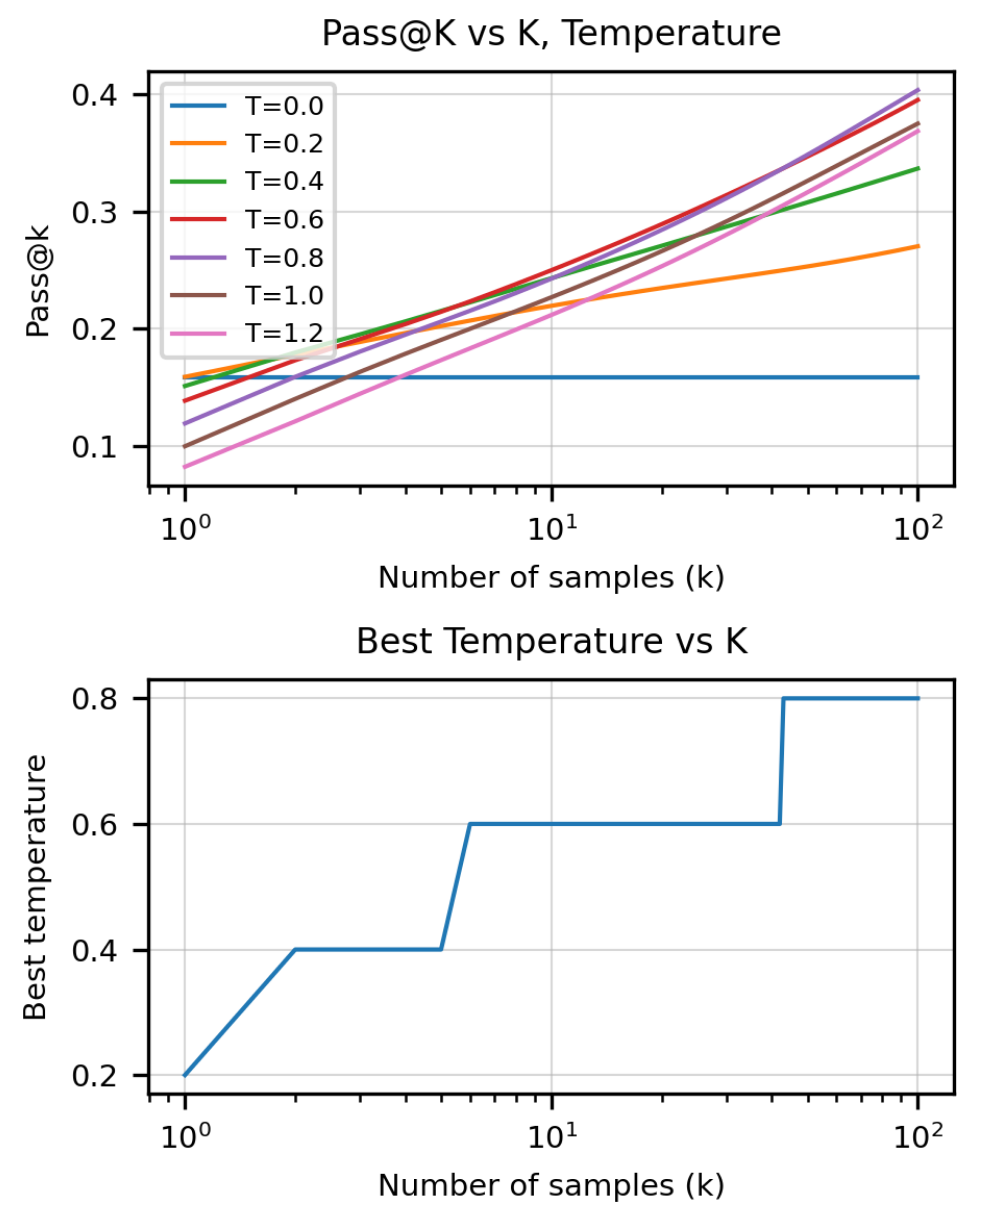
\includegraphics[width=0.5\linewidth]{PassVsK.png}
    \caption{Vergleich von $k$ aus der pass@k Metrik gegen die \texttt{temperature} des LLMs. Entnommen aus \cite{chenEvaluatingLargeLanguage2021}.}
    \label{fig:Pass vs K}
\end{figure}

\subsection{Weitere Konfigurationsparameter}\label{ch:Versuchsaufbau:Weitere Konfig}

Neben der Konfiguration des LLMs ist auch die generelle Konfiguration der Experiment-Durchläufe relevant. Zuerst gillt klar zu stellen, dass diese Arbeit nicht den Rahmen hat um eine hohe Menge an Experiment-Durchläufen durchzuführen. Aus diesem Grund ist die Menge an Durchläufen für 1 Code-Generierungslösung x 1 Benchmark $n=1$.

Aus dieser Restriktion folgt auch eine Konsequenz für die zu meldende Metrik. für $pass@k$ mit einem $k=1$ und einem $n=1$ kollabiert die gegebene Formel aus \todo{ref} zu einem einfachen $c/n$, also dem Durchschnitt. Daher werden die Ergebnisse in $avg@1$ gemeldet.

\subsubsection{Agentische Limits}

Agentische Systeme die in dieser Arbeit getestet werden können die Menge an erlaubten Schritten konfigurieren. Diese werden daher möglichst gleichmäßig konfiguriert. Dies bedeutet im Detail:

\begin{itemize}
    \item \textbf{CodeTeam} erlaubt die Konfiguration der kompletten Entwicklugnsrunden und der jeweiligen Schritte des Codes \& des Analyzers. \\ \todo{Schritte aus Arbeit übernehmen}
    \item \textbf{Terminus-2} erlaubt die Konfiguration der kompletten Schritte des Agenten. Da es sich hier um einen einzelnen Agenten handelt, wird die Schrittmenge auf $75$\todo{!} gesetzt.
\end{itemize}

\section{Durchführung und Abweichungen}\label{ch:Durchführung und Abweichungen}

Diese Sektion beschreibt den Prozess der Durchführung für die einzelnen Experimente.

\subsection{Vergleich Paper gegen Orchestrator}

Zunächst erfolgt die Durchführung mit der etabliert werden soll, inwiefern die Evaluierungs Plattform in ihren Ergebnissen von denen der Original-Paper abweicht.

\subsubsection{Self Collaboration}

Self Collaboration wird wie im Original Paper \cite{dongSelfCollaborationCodeGeneration2024} durchgeführt. Dies bedeutet die Evaluierung gegen den HumanEval Benchmark mit folgenden Hyperparametern:

\begin{itemize}
    \item \texttt{temperture = 0}
    \item \texttt{top\_p = 0.95}
    \item \texttt{max \_tokens = 512}
\end{itemize}

Das Original Paper nutze das Model \texttt{gpt-3.5-turbo-0301}. Dieses Modell wurde bereits vor Ende des Jahres 2024 eingestellt \cite{DeprecationsOpenAIAPI}. Es wurde daher die Entscheidung getroffen ein abweichendes Modell zu nutzen. Die Wahl viel hier auf \texttt{gpt-3.5-turbo-0613}. Es muss erwähnt werden dass dieses Modell vergleichsweise neuer ist, es kann davon ausgegangen werden dass es also leistungsfähiger ist.

Weitere Parameter, spezifisch für diesen Durchlauf sind wie folgt:

\begin{itemize}
    \item Maximum Runden zwischen Coder und Tester: 4
    \item Maximum Schritte für jeden Coder: 10
\end{itemize}

\section{Einordnung gegenüber publizierten Ergebnissen}\label{Einordnung gegenüber publizierten Ergebnissen}

Zunächst muss die Frage geklärt werden, welche Ergebnisse sich aus den Experimenten ergeben haben, die publizierte Ergebnisse nachstellen sollten. Daraus lässt sich später schlussfolgern ob die selbst gebaute Evaluierungs Plattform die gegebenen Ansätze so nutzt wie es die Authoren intendiert haben.

\subsection{Self Collaboration}

Wie bereits beschrieben, musste die lokale Ausführung leider auf ein neueres Modell ausweichen, da das originelle Modell nicht mehr verfügbar ist. Dennoch soll hier verglichen werden:

\begin{table}[H]
    \centering
    \caption{Vergleich Original Paper \& Evaluierungsplattform gegen HumanEval Benchmark}
    \label{tab:humaneval_comparison}
    \begin{tabular}{@{}lcc@{}}
        \toprule
        Ansatz & HumanEval & HumanEval-ET \\
        \midrule
        Original Paper & 74.4\% & 56.1\% \\
        Evaluierungs Plattform & 91.5\% & 79.3\% \\
        \bottomrule
    \end{tabular}
\end{table}

Ersichtlich ist, dass die lokale Implementierung in der Evaluierungs Plattform bessere Ergebnisse erzielt hat. Dies lässt sich durch die Nutzung eines anderen Modells erklären.

Unabhängig davon etabliert dies die Tatsache, dass die lokale Implementierung funktionsfähig ist. Ergebnisse sind in diesem Falle besser als die der originellen Publikation \cite{dongSelfCollaborationCodeGeneration2024}.

\section{Ergebnisse}\label{ch:Ergebnisse}



\section{Weitere Beobachtungen}\label{ch:Weitere Beobachtungen}

\todo[inline]{Falls relevant könnte man hier Randinformation mit aufnehmen, also Laufzeiten, Token Kosten, Iterationen (Harness), solche Sachen halt}

\section{Zusammenfassung}\label{ch:Zusammenfassung}


\controlquestions{
Im Kapitel „Experimente / Verifikation / Test / Validierung“ einer Abschlussarbeit wird überprüft, ob die entwickelte Lösung, das System oder das Konzept den Anforderungen genügt und die Forschungsfrage(n) beantwortet werden können. 
Dieses Kapitel ist zentral für die Beurteilung der Qualität, Aussagekraft und Belastbarkeit der Arbeitsergebnisse.
\begin{enumerate}
    \item Wurde direkt aus den Forschungsfragen (bzw. abgeleiteten Unterfragen, vgl.~Kapitel \ref{ch:Motivation und Problemdefinition}) und den Anforderungen bzw. Konzept (vgl.~Kapitel \ref{ch:Anforderungen und Konzept}) hergeleitet, warum ein Experiment nötig ist und was dieses nachweisen wird?
    \item Ist klar formuliert, was mit den Experimenten bzw. Tests überprüft oder validiert werden soll?
    \item Wurde das Experiment valide durchgeführt (mit ausführlicher Begründnung)? Z.~B.:
        \begin{itemize}
            \item mit verschiedenen Werten?
            \item mit ausreichenden Wiederholungen?
            \item in einer definierten, stabilen Umgebung?
            \item mit dokumentierten Parametern (Wiederholbarkeit/Reproducability)?
        \end{itemize}
    \item Sind gewählte Metriken, Messgrößen oder Bewertungskriterien nachvollziehbar und sinnvoll?
    \item Ist der Aufbau der Experimente methodisch korrekt und reproduzierbar dokumentiert?
    \item Wird das Vorgehen bei der Durchführung (z.\,B.~Testfälle, Abläufe) ausreichend detailliert beschrieben?
    \item Würde eine Wiederholung des Vorgehens zu ähnlichen Ergebnissen führen?
    \item Wurden Testdaten begründet ausgewählt oder erstellt – und sind diese ggf. dokumentiert/verfügbar?
    \item Werden die Ergebnisse verständlich, differenziert und strukturiert dargestellt (z.\,B.~mit Tabellen, Diagrammen, Text)?
    \item Sind die Ergebnisse vollständig dokumentiert – nicht nur die erfolgreichen, sondern auch unerwartete oder problematische?
    \item Sind die Messergebnisse mit geeigneten Methoden ausgewertet (z.\,B.~statistisch, vergleichend)?
    \item Gibt es einen Vergleich/Einordnung mit bestehenden Ansätzen, Referenzwerten oder einer Baseline?
    \item Wurde auf Reproduzierbarkeit und Generalisierbarkeit eingegangen?
    \item Beantworten die Ergebnisse die aufgestellten Forschungsfragen oder Zielsetzungen?
\end{enumerate}
}

\chapter{Diskussion}\label{ch:Diskussion}

\section{Interpretation der Ergebnisse}\label{ch:Diskussion:Interpretation der Ergebnisse}

\section{Einordnung gegenüber publizierten Ergebnissen}\label{ch:Diskussion:Einordnung gegenüber publizierten Ergebnissen}

\section{Threats to Validity}\label{ch:Diskussion:Threats to Validity}

\section{Belastbarkeit der Ergebnisse}\label{ch:Diskussion:Belastbarkeit der Ergebnisse}

\section{Implikationen und Handlungsempfehlungen}\label{ch:Diskussion:Implikationen und Handlungsempfehlungen}

\section{Offene Fragen}\label{ch:Diskussion:Offene Fragen}

\controlquestions{
Dieses Kapitel in einer Abschlussarbeit ist zentral, um die Ergebnisse einzuordnen, kritisch zu reflektieren und sie in einen größeren wissenschaftlichen Kontext zu stellen. 
Hier wird gezeigt, dass die forschende Person Arbeitsergebnisse nicht nur präsentieren, sondern auch durchdenken,  qualifiziert einordnen und bewerten kann.
\begin{itemize}
    \item Interpretation und Bewertung der Ergebnisse
        \begin{enumerate}
            \item Werden die Ergebnisse kritisch interpretiert – auch in Hinblick auf die gestellten Anforderungen oder Hypothesen?
            \item Wird erklärt, was die Ergebnisse bedeuten – im Lichte der Zielsetzung, Hypothesen oder Erwartungen?
            \item Wird zwischen objektiven Befunden und subjektiver Interpretation (persönliche Bewertung) klar unterschieden?
            \item Wird erkennbar, ob und wie gut das entwickelte System/Konzept den Anforderungen gerecht wird?
            \item Werden die zentralen Ergebnisse sinnvoll zusammengefasst – ohne sie einfach zu wiederholen?
            \item Wurde klar zwischen Korrelation und Kausalität unterschieden?
        \end{enumerate}
    \item Reflexion von Unsicherheiten und Einschränkungen
        \begin{enumerate}[resume]
            \item Werden mögliche Fehlerquellen, Unsicherheiten oder Einschränkungen der Ergebnisse reflektiert?
            \item Wurden unerwartete oder widersprüchliche Ergebnisse angesprochen und erklärt?
            \item Wird die Zuverlässigkeit und Aussagekraft der Ergebnisse eingeschätzt?
            \item Sind methodische Schwächen oder Einschränkungen der Arbeit ehrlich und sachlich reflektiert?
            \item Ist transparent, was methodisch nicht optimal gelöst werden konnte – und warum?
            \item Wird die Einschätzung der Bedrohungen sachlich, reflektiert und ohne Beschönigung dargestellt?
            \item Wird klar, wie stark die Ergebnisse trotz der \emph{Threats of Validity} belastbar sind?
        \end{enumerate}
    \item Einordnung im wissenschaftlichen Kontext
        \begin{enumerate}[resume]
            \item Werden die Ergebnisse in Bezug zu bestehender Literatur oder Theorien (vgl.~Kapitel \ref{ch:Verwandte Arbeiten}) gesetzt?
            \item Wird erläutert, inwiefern die Ergebnisse bestehende Ansätze stützen, erweitern oder widersprechen?
            \item Werden relevante wissenschaftliche Kontroversen oder alternative Erklärungen aufgegriffen?
            \setcounter{lastenumcounter}{\value{enumi}}
        \end{enumerate}
\end{itemize}
}
\controlquestionscontinue{
\begin{itemize}
    \item Praktische und theoretische Implikationen
        \begin{enumerate}\setcounter{enumi}{\value{lastenumcounter}}
            \item Ergeben sich aus den Ergebnissen Handlungsempfehlungen, Optimierungspotenzial oder weitere Fragestellungen?
            \item Welche praktischen, wissenschaftlichen oder gesellschaftlichen Konsequenzen lassen sich aus den Ergebnissen ableiten?
            \item Gibt es Handlungsempfehlungen oder Hinweise für die Anwendung in der Praxis und/oder weiteren Forschung?
        \end{enumerate}
    \item Überleitung zu Ausblick und zukünftige Arbeiten
        \begin{enumerate}[resume]
            \item Welche offenen Fragen bleiben bestehen?
            \item Welche Ansätze zur Weiterentwicklung oder für zukünftige Forschung ergeben sich?
            \item Wird die Diskussion schlüssig abgeschlossen und ein Übergang zum Fazit (vgl.~Kapitel \ref{ch:Zusammenfassung und zukünftige Arbeiten}) geschaffen?
        \end{enumerate}
    \item Threats to Validity
        \begin{enumerate}[resume]
            \item Gab es Störfaktoren, die das Ergebnis beeinflusst haben könnten (z.\,B.~Lernkurveneffekte, unbeachtete Variablen)?
            \item Wurden potenzielle Bias (z.\,B.~durch Auswahl der Probanden, Messinstrumente) reflektiert?
            \item Ist die Stichprobe (z.\,B.~Personen, Daten, Testfälle) repräsentativ genug für eine Verallgemeinerung?
            \item Wird erklärt, in welchen Kontexten die Ergebnisse nicht ohne Weiteres gelten?
            \item Sind die Rahmenbedingungen der Untersuchung möglicherweise so speziell, dass sie die Übertragbarkeit einschränken?
        \end{enumerate}
\end{itemize}
}



\chapter{Zusammenfassung und zukünftige Arbeiten}\label{ch:Zusammenfassung und zukünftige Arbeiten}

\lipsum[15-16] % remove

\controlquestions{
Dieses Kapitel soll die wichtigsten Erkenntnisse klar und prägnant zusammenfassen und einen Ausblick auf mögliche Weiterentwicklungen oder offene Fragestellungen geben.
\begin{itemize}
    \item Fazit:
        \begin{enumerate}
            \item Wird die zentrale Forschungsfrage noch einmal klar benannt?
            \item Sind die wichtigsten Ergebnisse und Erkenntnisse verständlich und prägnant zusammengefasst – ohne Wiederholung ganzer Passagen?
            \item Wird nachvollziehbar gezeigt, inwiefern die Ziele der Arbeit erreicht wurden?
            \item Wird klar, wie die Arbeit zum Stand der Forschung und/oder Praxis beiträgt?
            \item Werden keine neuen Inhalte oder Details eingeführt?
            \item Ist die Zusammenfassung kompakt, aber dennoch inhaltlich vollständig?
            \item Wird ein klarer, reflektierter letzter Eindruck hinterlassen?
            \item Sind alle Aspekte des Abstracts und des Kapitels “Motivation” gespiegelt, d.\,h.~alle dort erwähnten Themen/Punkte werden nun aus dem Blickpunkt der abgeschlossenen Arbeit erneut dargestellt?
        \end{enumerate}
    \item Zukünftige Arbeiten:
        \begin{enumerate}
            \item Wurden im Ausblick die (wichtigsten) sich neu ergebenen wissenschaftlichen Fragestellungen besprochen?
            \item Wurden realistische und relevante Vorschläge für weiterführende Arbeiten gemacht?
            \item Wurde begründet, warum bestimmte Aspekte oder Fragestellungen in künftiger Forschung weiterverfolgt werden sollten?
            \item Wurde reflektiert, welche Limitationen der Arbeit zu weiterem Forschungsbedarf führen?
            \item Sind die vorgeschlagenen zukünftigen Arbeiten konkret (z.\,B.~methodisch, thematisch oder technisch eingegrenzt)?
        \end{enumerate}
\end{itemize}

}



% --------------------------
% Back matter
% --------------------------
%
{%
\setstretch{1.1}
\renewcommand{\bibfont}{\normalfont\small}
\setlength{\biblabelsep}{0.25em}
\setlength{\bibitemsep}{0.5\baselineskip plus 0.5\baselineskip}
% print all references that are not ot type online
\printbibliography[nottype=online]
\newrefcontext[labelprefix={@}]
% web pages are typically non-scientific resources, so we separate them from the scientific ones
% typically 
\printbibliography[heading=subbibliography,title={Webpages},type=online]

\todo[inline,color=red]{Warnung: es fehlt in der Darstellung der Referenzen ein Wert wie "Access on: xx.xx.yyyy", was bei den websiten ungünstig ist (WSE Referenz kann nicht durch waybackmachine erhalten werden...)}

\todo[inline]{Nochmal checken warum bei den waybackmachine links kein Zeilenumbruch stattfindet}

\controlquestions{
\begin{enumerate}
    \item Sind alle Quellen an den relevanten Stellen im Text angegeben?
    \item Ist das Literaturverzeichnis vollständig? 
    \item Sind die Begriffe im Titel der Arbeit korrekt geschrieben (QALD, nicht qald; IBM, nicht ibm; DBpedia, nicht dbpedia; GitHub, nicht github; etc.)
    \item Sind wissenschaftliche Quellen vollständig angegeben (alle Autoren, Konferenz/Journal, DOI, etc.)?
    \item Sind alle Online-Quellen mit dem Datum des letzten Abrufs versehen und klar referenzierbar?
    \item Sind die URLs für alle Online-Quellen unveränderlich (Beispiel: GitHub-URLs mit Hash, Wikipedia-Seiten mit Zeitstempel)? Sind alle anderen Webseiten über \url{https://web.archive.org/} persistiert und im BibTeX anstatt der Original-URL referenziert?  
\end{enumerate}
}
}
\cleardoublepage

\listoffigures
\cleardoublepage

\listoftables
\cleardoublepage

%\lstlistoflistings
%\cleardoublepage

\appendix\cleardoublepage
% !TEX root = ../my-thesis.tex
%
\chapter{Appendix}\label{sec:appendix}

% Style für prompt Darstellung
\lstdefinestyle{promptstyle}{
  basicstyle=\ttfamily\footnotesize,
  columns=fullflexible,
  keepspaces=true,
  upquote=true,
  showstringspaces=false,
  breaklines=true,
  breakindent=0pt,
  breakautoindent=false,
  postbreak=\mbox{\textcolor{gray}{$\hookrightarrow$}\space},
  frame=single,
  rulecolor=\color{gray!50},
  xleftmargin=0pt,
  numbers=none,
  captionpos=b,
}

\section{Single-Shot Prompt}\label{sec:appendix:single-shot-prompt}

\begin{lstlisting}[style=promptstyle,
                   caption={Ausgabeprotokoll der Single-Shot-Solution
                            (Python-Konstante \texttt{FORMAT\_INSTRUCTION});
                            wird der Task-Beschreibung unverändert angehängt.},
                   label={lst:prompt-singleshot}]
Write out the complete project, one file at a time. Introduce each file with a
line naming its path, then give that file's entire contents in a fenced code
block:

### FILE: src/example/core.py
```python
def add(left: int, right: int) -> int:
    return left + right
```

- Paths are relative to the project root: `pyproject.toml` belongs at
  `pyproject.toml`, not inside a directory named after the project.
- Where the specification shows a directory tree, its top-level directory is
  the project root itself and not a directory to create.
- No absolute paths, and no `..`.
- Include every file the project needs in order to be installed and used,
  packaging and configuration among them.
- Write each file out in full. Do not abbreviate a body to a comment, and do
  not leave a placeholder to be filled in later.
- If a file's own contents contain a fenced code block, fence that file with
  more backticks than appear anywhere inside it.
- Only the file blocks are read. Any other text is ignored.
\end{lstlisting}       % INCLUDE: appendix

%\cleardoublepage
%\input{content/colophon}

%\cleardoublepage
%\input{content/declaration}
%\clearpage

%\newpage
\mbox{}

% **************************************************
% End of Document CONTENT
% **************************************************
\end{document}
